\documentclass[11pt,letterpaper,english]{article}

\usepackage[T1]{fontenc}
\usepackage[utf8]{inputenc}
\usepackage[english]{babel}
\usepackage[margin=1in]{geometry}
\usepackage[numbers]{natbib}
\setcitestyle{nocompress}
\bibpunct{(}{)}{;}{a}{}{,}

% \usepackage[nocompress]{cite}
\usepackage{graphicx}
\usepackage[cmex10]{amsmath}
\usepackage{authblk}
\usepackage{macros}
\newtheorem{corollary}[theorem]{Corollary}

\begin{document}
\title{Cumulative Prospect Theory Meets Reinforcement Learning: Prediction and Control}

\author[1]{Prashanth L.A.\thanks{prashla@isr.umd.edu}}
\author[2]{Cheng Jie\thanks{cjie@math.umd.edu}}
\author[3]{Michael Fu\thanks{mfu@isr.umd.edu}}
\author[4]{Steve Marcus\thanks{marcus@umd.edu}}
\author[5]{Csaba Szepesv\'ari\thanks{szepesva@cs.ualberta.ca}}
\affil[1]{\small Institute for Systems Research, University of Maryland}
\affil[2]{\small Department of Mathematics, University of Maryland}
\affil[3]{\small Robert H. Smith School of Business \& Institute for Systems Research,
University of Maryland}
\affil[4]{\small Department of Electrical and Computer Engineering \& Institute for Systems Research,
University of Maryland}
\affil[5]{\small Department of Computing Science,
University of Alberta}

\renewcommand\Authands{ and }

\date{}

\maketitle

\begin{abstract}
Cumulative prospect theory (CPT) is known to model human decisions well, with substantial empirical evidence supporting this claim. 
CPT works by distorting probabilities and is more general than the classic expected utility and coherent risk measures. We bring this idea to a risk-sensitive reinforcement learning (RL) setting and design algorithms for both estimation and control.
The RL setting presents two particular challenges when CPT is applied: estimating the CPT objective requires estimations of the {\it entire distribution} of the value function and finding a {\it randomized} optimal policy.
The estimation scheme that we propose uses the empirical distribution to estimate the CPT-value of a random variable. We then use this scheme in the inner loop of policy optimization procedures for a stochastic shortest path problem. 
We propose both gradient-based as well as gradient-free policy optimization algorithms. The former includes both first-order and second-order methods that are based on the well-known simulation optimization idea of simultaneous perturbation stochastic approximation (SPSA), while the latter is based on a reference distribution that concentrates on the global optima. Using an empirical distribution over the policy space in conjunction with  Kullback-Leibler (KL) divergence to the reference distribution, we get a global policy 
optimization scheme.
We provide theoretical convergence guarantees for all the proposed algorithms and also empirically demonstrate the usefulness of our algorithms. 
\end{abstract}

% \keywords{
% Cumulative prospect theory, reinforcement learning, Service systems,  labor optimization, Adaptive labor staffing, Simultaneous
% perturbation stochastic approximation.
% }



\section{Introduction}
\label{sec:introduction}
Risk-sensitive reinforcement learning (RL) has received a lot of attention recently (cf. \cite{borkar2010learning,borkar2010risk,tamar2012policy,Prashanth13AC}). Previous works consider either an exponential utility formulation (cf. \cite{borkar2010learning}) that implicitly controls the variance or a constrained formulation with explicit constraints on the variance of the cost-to-go (cf. \cite{tamar2012policy,Prashanth13AC}). Another constraint alternative is to bound a coherent risk measure such as Conditional Value-at-Risk (CVaR), while minimizing the usual cost objective (cf. \cite{borkar2010risk,prashanth2014policy}).  

In several real-world systems involving humans, traditional expected utility and risk-sensitive control approaches cannot explain the observed behavior as humans are not rational/consistent. In other words, for a human there do not exist utility functions whose expectation can be maximized nor coherent measures such as CVaR fit well with human preferences. This problem can be alleivated by incorporating distortions in the underlying probabilities of the system. Probabilistic distortions have a long history in behavioral science and economics and a very popular approach comes from \textit{Prospect Theory (PT)} \cite{kahneman1979prospect} and its later enhancement \textit{cumulative prospect theory} (CPT) \cite{tversky1992advances}. 

%\pgfkeyssetvalue{/cfr/soul base dimension}{5pt}
%\begin{tikzpicture}
  %[
  %font=\sffamily\bfseries,
  %line width=0.1*\pgfkeysvalueof{/cfr/soul base dimension},
  %outer sep=0pt,
  %inner sep=0pt,
  %person/.pic={%
    %\node (-head) [circle, minimum size=4*\pgfkeysvalueof{/cfr/soul base dimension}] {};
    %\node (-torso) [below=0pt of -head, rectangle, rounded corners=.4*\pgfkeysvalueof{/cfr/soul base dimension}, minimum width=3.5*\pgfkeysvalueof{/cfr/soul base dimension}, minimum height=6*\pgfkeysvalueof{/cfr/soul base dimension}] {};
    %\node (-right arm) [right=0pt of -torso.north east, yshift=-3.1*\pgfkeysvalueof{/cfr/soul base dimension}, rectangle, minimum width=\pgfkeysvalueof{/cfr/soul base dimension}, minimum height=6*\pgfkeysvalueof{/cfr/soul base dimension}, rounded corners=.4*\pgfkeysvalueof{/cfr/soul base dimension}] {};
    %\node (-left arm) [left=0pt of -torso.north west, yshift=-3.1*\pgfkeysvalueof{/cfr/soul base dimension}, rectangle, minimum width=\pgfkeysvalueof{/cfr/soul base dimension}, minimum height=6*\pgfkeysvalueof{/cfr/soul base dimension}, rounded corners=.4*\pgfkeysvalueof{/cfr/soul base dimension}] {};
    %\node (-left leg) [below=0pt of -torso.south, rectangle, minimum width=1.5*\pgfkeysvalueof{/cfr/soul base dimension}, minimum height=6*\pgfkeysvalueof{/cfr/soul base dimension}, rounded corners=.2*\pgfkeysvalueof{/cfr/soul base dimension}, anchor=north east] {};
    %\node (-right leg) [below=0pt of -torso.south, rectangle, minimum width=1.5*\pgfkeysvalueof{/cfr/soul base dimension}, minimum height=6*\pgfkeysvalueof{/cfr/soul base dimension}, rounded corners=.2*\pgfkeysvalueof{/cfr/soul base dimension}, anchor=north west] {};
    %\draw [rounded corners=.2*\pgfkeysvalueof{/cfr/soul base dimension}] (-right leg.south) -- (-right leg.south west) -- (-left leg.south east) -- (-left leg.south west)  -- (-torso.south west) [rounded corners=.4*\pgfkeysvalueof{/cfr/soul base dimension}] -- (-left arm.south east) -- (-left arm.south west) -- (-left arm.north west) -- (-torso.north west) -- ($(-head.south) - (.5*\pgfkeysvalueof{/cfr/soul base dimension},0)$) arc [start angle=255.5, end angle=-74.5, radius=2*\pgfkeysvalueof{/cfr/soul base dimension}] -- (-torso.north east) -- (-right arm.north east) -- (-right arm.south east)  -- (-right arm.south west) [rounded corners=.2*\pgfkeysvalueof{/cfr/soul base dimension}] -- (-torso.south east)  -- (-right leg.south east) -- (-right leg.south west);
  %}
  %]
  %\thetac (feeling small) [fill=red,blue] {person};
%\end{tikzpicture}

\tikzset{
  pobl/.style={
    inner sep=0pt, outer sep=0pt, fill=#1,
  },
  pobl gron/.style n args={2}{
    pobl=#1, rounded corners=#2,
  },
  pics/person/.style n args={3}{
    code={
      \node (-corff) [pobl=#1, minimum width=.25*#2, minimum height=.375*#2, rotate=#3, pic actions] {};
      \node (-pen) [minimum width=.3*#2, circle, pobl=#1, outer sep=.01*#2, anchor=south, rotate=#3, pic actions] at (-corff.north) {};
      \node (-coes dde) [pobl gron={#1}{1pt}, anchor=north west, minimum width=.12125*#2, minimum height=.25*#2, rotate=#3, pic actions] at (-corff.south west) {};
      \node [pobl=#1, anchor=north, minimum width=.12125*#2, minimum height=.15*#2, rotate=#3, pic actions] at (-coes dde.north) {};
      \node (-coes chwith) [pobl gron={#1}{1pt}, anchor=north east, minimum width=.12125*#2, minimum height=.25*#2, rotate=#3, pic actions] at (-corff.south east) {};
      \node [pobl=#1, anchor=north, minimum width=.12125*#2, minimum height=.15*#2, rotate=#3, pic actions] at (-coes chwith.north) {};
      \node (-braich dde) [pobl gron={#1}{.75pt}, minimum width=.075*#2, minimum height=.325*#2, outer sep=.0064*#2, anchor=north west, rotate=#3, pic actions] at (-corff.north east)  {};
      \node [pobl=#1, minimum width=.05*#2, minimum height=.2*#2, outer sep=.0064*#2, anchor=north west, rotate=#3, pic actions] at (-corff.north east) {};
      \node (-braich chwith) [pobl gron={#1}{.75pt}, minimum width=.075*#2, minimum height=.325*#2, outer sep=.0064*#2, anchor=north east, rotate=#3, pic actions] at (-corff.north west) {};
      \node [pobl=#1, minimum width=.0375*#2, minimum height=.2*#2, outer sep=.0064*#2, anchor=north east, rotate=#3, pic actions] at (-corff.north west) {};
      \node (-fit person) [fit={(-pen.north) (-braich dde.east) (-coes chwith.south) (-braich chwith.west)}] {};
      %\node (-pwy) [below=25pt of -fit person, every pin] {\tikzpictext};
      %\draw [every pin edge] (-fit person) -- (-pwy);
    },
  },
}
\tikzstyle{block} = [draw, fill=white, rectangle,
   minimum height=3em, minimum width=6em]
\tikzstyle{sum} = [draw, fill=white, circle, node distance=1cm]
\tikzstyle{input} = [coordinate]
\tikzstyle{output} = [coordinate]
\tikzstyle{pinstyle} = [pin edge={to-,thin,black}]

\begin{figure}[h]
\centering
\scalebox{0.85}{\begin{tikzpicture}[auto, node distance=2cm,>=latex',
    every pin edge/.append style={latex-, shorten <=-2.5pt}
  ]
\node [block,fill=blue!20, minimum height=4em,] (world) {\makecell{\large\bf World}}; 
\node [block,fill=red!20, below=2.5cm of world] (agent) {\makecell{\large\bf Agent}}; 
\node [circle,fill=brown!50!black,right=2cm of world,label=above:{\bf Reward}] (tmp) {};
\coordinate [below left=2.5cm of world] (tmp2);
\coordinate [below right=1cm of agent] (belowagent);

\draw [->,thick] (world)  -| (tmp) |-   (agent);
\draw [->,thick] (agent)  -| (tmp2) |-   (world);
%\draw [->] (agent) --   (world);
\draw pic (person)  [right =3cm of tmp] {person={blue}{50pt}{0}};
\coordinate [right=2.8cm of tmp] (tmp3);
\coordinate [below right=16pt of tmp3] (tmp4);
\draw [->,thick] (tmp) --   (tmp3);
\draw [->,thick,dotted] (tmp4)  |- node[below left=0.1cm and 1cm] {\textbf{CPT model parameters}} (belowagent) -|  (agent.south);
\end{tikzpicture}}
\caption{Operational flow of a human-based decision making system}
\label{fig:flow}
\end{figure}
%\begin{tikzpicture}
  %[
    %every pin edge/.append style={latex-, shorten <=-2.5pt},
  %]

As illustrated in Figure \ref{fig:flow}, we consider a typical RL setting where the environment is unknown, but can be experimented with and propose a CPT based risk measure as the long-term performance objective. 
CPT is a non-coherent and non-convex measure that is well known among psychologists and economists to be a good model for human decision-making systems, with strong empirical support.
To put it differently, CPT captures well the way humans evaluate outcomes and hence, we offer a CPT-variant of the RL notion of ``value function''. Unlike the regular value function which is the expectation of the return random variable, CPT-value employs a functional that distorts the underlying probabilities. The latter is achieved by fitting CPT model parameters to capture human preferences. The goal then for the learning system is to find a policy that maximizes the CPT-value of ``return''. 

%
%In the realm of sequential decision making under uncertainty, we propose a CPT-based risk measure.  In particular,  
%The current RL solutions cannot handle distortions and my current work is to develop both prediction and control schemes for probabilistically distorted MDPs.
%
%\todop[inline]{Add refs for distorted weights}
%In this paper, we consider a risk measure based on \textit{cumulative prospect theory} (CPT) \cite{tversky1992advances}, which is a non-coherent and non-convex measure that is well known among psychologists and economists to be a good model for human decision-making systems, with strong empirical support. In this paper, we incorporate CPT-based criteria into the classic objective \textit{value function} in a reinforcement learning framework. Intuitively this combination is appealing because it taps into the notion of how humans evaluate outcomes and also, a CPT objective leads to a randomized policy, which although harder to estimate often leads to more intuitively appealing behavior, as illustrated via an example below and also the numerical experiments later.

%%%%%%%%%%%%
In terms of research contributions, this is the first work to combine CPT with RL, and although on the surface it might seem straightforward, in fact there are many research challenges that arise from trying to apply a CPT objective in the RL framework. \\
\textbf{Prediction:} In the case of the classic value function, which is an expectation, a simple sample means can be used for estimation, facilitating the use of temporal difference type algorithms. On the other hand, estimating the CPT-value for a given policy is challenging, because it requires that the \textit{entire} distribution of the total cost to be estimated.\\ 
\textbf{Control:} 
Designing policy optimization algorithms in order to find a \textit{CPT-optimal} policy is challenging because CPT-value is a non-coherent and non-convex risk measure that does not lend itself to dynamic programming approaches such as value/policy iteration due to the lack of a ``Bellman equation''. Thus, it is necessary to design new simulation optimization scheme that use sample CPT-value estimates to optimize the policy, which is generally \textit{randomized}. 

To put things in context, risk-sensitive reinforcement learning problems are generally hard to solve. 
For a discounted MDP, \cite{Sobel82VD} showed that there exists a Bellman equation for the variance of the return, but the underlying Bellman operator is not necessarily monotone. The latter observation rules out policy iteration as a solution approach for variance-constrained MDPs.
Further, even if the transition dynamics are known, \cite{mannor2013algorithmic} show that finding a globally mean-variance optimal policy in a discounted MDP is NP-hard.
For average reward MDPs, \cite{filar1989variance} consider a variance definition that measures how far the instantaneous reward is away from its average, unlike the discounted setting where the variance was of the return r.v. However, for average reward MDPs, \cite{filar1989variance} motivate their variance definition well and then provide NP-hardness results for finding a globally optimal policy with the variance constraint.
CVaR as a risk measure is equally (if not more) complicated as the measure here is a conditional expectation, where the conditioning is on a low probability event. Apart from the hardness of finding CVaR-optimal solutions, estimating CVaR for a fixed policy in a typical RL setting itself is a challenge considering CVaR relates to rare events and to the best of our knowledge, there is no algorithm with theoretical guarantees to estimate CVaR without wasting a lot of samples. There are proposals based on importance sampling (cf. \cite{prashanth2014policy,tamar2014optimizing}), but they lack theoretical guarantees. In contrast, we derive a \textit{provably} sample-efficient scheme for estimating the CPT-value (see next section for a precise definition) for a given policy and use this as the inner loop in a policy optimization schemes that include gradient-based as well as gradient free approaches. Finally, we point out that the CPT-value that we define is a generalization in the sense that one can recover the regular value function and the risk measures such as VaR and CVaR by appropriate choices of a certain weight function used in the definition of CPT value (see the next section for precise details).

The rest of the paper is organized as follows: 
In Section~\ref{sec:cpt-val}, we introduce the notion of CPT-value of a general random variable $X$ and make a special case illustration when $X$ is the return of a stochastic shortest path problem.
In Section~\ref{sec:cpt-sampling}, we
describe the empirical distribution based scheme for estimating the CPT-value of any random variable. In Sections \ref{sec:1spsa}--\ref{sec:2spsa}, we present the gradient-based algorithms for optimizing the CPT-value. Next, in Section \ref{sec:mras}, we present a gradient-free model-based algorithm for CPT-value optimization in an MDP. We provide the proofs of convergence for all the proposed algorithms in Section~\ref{sec:convergence}.
We present the results from numerical experiments for the CPT-value estimation scheme in Section~\ref{sec:expts} and finally, provide the concluding remarks in Section~\ref{sec:conclusions}.

%%%%%%%%%%%%%5
\section{CPT-value}
\label{sec:cpt-val}
For a real-valued random variable $X$, we first introduce a ``CPT-functional'' the replaces the traditional expectation. Subsequently, we specialize $X$ to be the return of stochastic shortest path problem.
\subsection{General definition}
The CPT-value of the random variable $X$ is a functional defined as
\begin{align}
\C_{u,w}(X) = &\intinfinity w^+(P(u^+(X))>z) dz - \intinfinity w^-(P(u^-(X))>z) dz, \label{eq:cpt-general}
\end{align}
where $u=(u^+,u^-)$, $w=(w^+,w^-)$, $u^+,u^-:\R\rightarrow \R_+$ and $w^+,w^-:[0,1] \rightarrow [0,1]$ are continuous (see assumptions (A1)-(A2) in Section \ref{sec:cpt-sampling} for precise requirements on the $u$ and $w$). For notational convenience, we drop the dependence on $u,w$ and use $\C(X)$ to denote the CPT-value.  

Let us deconstruct the above definition:
 \begin{figure}[h]
   \centering
\tabl{c}{
%\includegraphics[width=3.8in]{utility.png}}
   \scalebox{1.0}{\begin{tikzpicture}
   \begin{axis}[width=11cm,height=6.5cm,legend pos=south east,
          %  grid = major,         
            axis lines=middle,
           % grid style={dashed, gray!30},
            xmin=-5,     % start the diagram at this x-coordinate
            xmax=5,    % end   the diagram at this x-coordinate
            ymin=-4,     % start the diagram at this y-coordinate
            ymax=4,   % end   the diagram at this y-coordinate
           % axis background/.style={fill=white},
            ylabel={\large\bf Utility},
            xlabel={\large\bf Gains},
            x label style={at={(axis cs:4.7,-0.8)}},
            y label style={at={(axis cs:-0.8,4.8)}},
            xticklabels=\empty,
            yticklabels=\empty
            ]
           \addplot[name path=cptplus,domain=0:5, green!35!black, very thick,smooth] 
              {pow(abs(x),0.8)}; 
            \addplot[name path=cptminus,domain=-5:0, red!35!black,very thick,smooth] 
              {-2*pow(abs(x),0.7)}; 
               \addplot[domain=-5:5, blue, thick]           {x}; 
               
               \path[name path=diagplus] (axis cs:0,0) -- (axis cs:5,5);
 			  \path[name path=diagminus] (axis cs:-5,-5) -- (axis cs:0,0);
                \path[name path=xaxisplus] (axis cs:0,0) -- (axis cs:5,0);
                 \path[name path=xaxisminus] (axis cs:-5,0) -- (axis cs:0,0);
                 \path[name path=yaxisplus] (axis cs:0,0) -- (axis cs:0,5);
                 \path[name path=yaxisminus] (axis cs:0,-5) -- (axis cs:0,0);
 
 \addplot [orange!40]  fill between[of= diagminus and yaxisminus];
 \addplot [cyan!20]  fill between[of= diagplus and xaxisplus];
 
 \node at (axis cs:  -3.7,-0.45) {\large\bf Losses};
 \node at (axis cs:  4,2.5) {\large $\bm{u^+}$};
 \node at (axis cs:  -1,-3) {\large $\bm{u^-}$};
   \end{axis}
   \end{tikzpicture}}}\\[1ex]
\caption{Utility function}
\label{fig:u}
\end{figure}

\paragraph{Utility functions:} $u^+, u^-$ are utility functions corresponding to gains ($X \ge 0$) and losses ($X \le 0$), respectively. For example, consider a scenario where one can either earn \$$500$ w.p $1$ or earn \$$1000$ w.p. $0.5$ (and nothing otherwise). The human tendency is to choose the former option of a certain gain. If we flip the situation, i.e., a certain loss of \$$500$ or a loss of \$$1000$ w.p. $0.5$, then humans choose the latter option.  Handling losses and gains separately is a salient feature of CPT and this addresses the tendency of humans to play safe with gains and take risks with losses - see Fig \ref{fig:u}.  In contrast, the traditional value function makes no such distinction between gains and losses.  

\begin{figure}[h]
\centering
\tabl{c}{
%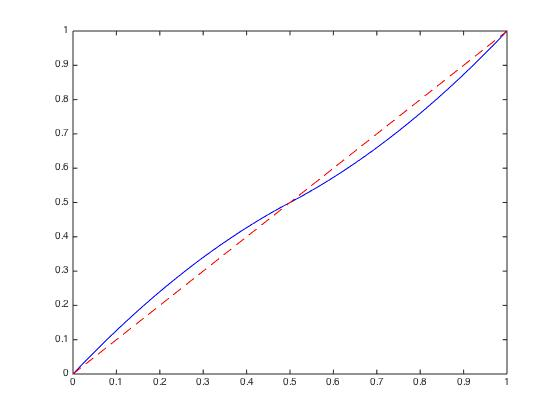
\includegraphics[width=8cm]{results/Probability_weighting_function.jpg}
  \scalebox{1.0}{\begin{tikzpicture}
  \begin{axis}[width=11cm,height=6.5cm,legend pos=south east,
           grid = major,
           grid style={dashed, gray!30},
           xmin=0,     % start the diagram at this x-coordinate
           xmax=1,    % end   the diagram at this x-coordinate
           ymin=0,     % start the diagram at this y-coordinate
           ymax=1,   % end   the diagram at this y-coordinate
           axis background/.style={fill=white},
           ylabel={\large Weight $\bm{w(p)}$},
           xlabel={\large Probability $\bm{p}$}
           ]
          \addplot[domain=0:1, red, thick,smooth,samples=1500] 
             {pow(x,0.6)/(pow(x,0.6) + pow(1-x,0.6))}; 
             \node at (axis cs:  0.8,0.35) (a1) {\large $\bm{\frac{p^{0.6}}{(p^{0.6}+ (1-p)^{0.6})}}$};           
             \draw[->] (a1) -- (axis cs:  0.7,0.6);
                 \addplot[domain=0:1, blue, thick]           {x};                      
  \end{axis}
  \end{tikzpicture}}\\[1ex]
}
\caption{Weight function}
\label{fig:w}
\end{figure}

\paragraph{Weight functions:} $w^+, w^-$ are functions corresponding to gains and losses, respectively. 
The main idea is that humans deflate high-probabilities and inflate low-probabilities and this is the rationale behind using a weight function in CPT.
For example, humans usually choose a stock that gives \$$10000$ w.p. $0.001$ over one that gives \$$10$ w.p. $1$ and the reverse when signs are flipped. 
Thus the value seen by the human subject is non-linear in the underlying probabilities - an observation with strong empirical evidence that used human subjects (see \cite{tversky1992advances} or $8000$+ papers that follow).  In contrast,the traditional value function is linear in the underlying probabilities. 
As illustrated with $w=w^+=w^-$ in Fig \ref{fig:w}, the weight functions are continuous, non-decreasing and have the range $[0,1]$ with $w^+(0)=w^-(0)=0$ and $w^+(1)=w^-(1)=1$. Weight functions can explain non-linear probability distortions, as illustrated by the following example: 
\begin{description}
 \item[\textit{[Stock 1]}] This investment results in a gain of \$$10$ with probability (w.p.) $0.1$ and a loss of \$$500$ w.p. $0.9$. The expected return is \$$-449$, but this does not necessarily imply that ``human'' investors' evaluation of the stock is \$$-449$. Instead, it is very likely that the humans evaluate it to a higher value, e.g. \$$-398$ ($=$ gain w.p. $0.2$ and loss w.p. $0.8$).\footnote{See Table 3 in \cite{tversky1992advances} to know why such a human evaluation is likely.}
\item[\textit{[Stock 2]}] loss of \$$10$ w.p. $0.9$, gain \$$500$ w.p. $0.1$. Expected return: \$$41$; Human evaluation: \$$92$ ($=$ loss w.p. $0.8$).
\item[\textit{[Stock 3]}] loss of \$$10$ w.p. 0.1, gain \$$500$ w.p. $0.9$. Expected return: \$$449$; Human evaluation: \$$398$ ($=$ loss w.p. $0.2$). 
\end{description}

\paragraph{Optimization objective:} Suppose the r.v. $X$ is a function of a $d$-dimensional parameter $\theta$. The goal then is to solve the following problem:
\begin{align}
\label{eq:opt-general}
\textrm{Find ~}\theta^* = \argmin_{\theta \in \Theta} \C(X^\theta),
\end{align}
where $\Theta$ is a compact and convex subset of $\R^d$.
The above optimization problem has several applications in RL. For instance, $X$ could be the total reward/discounted reward/average reward r.v. for a fixed policy (given as $\theta$) in the context of a stochastic shortest path/discounted/average reward MDP, respectively. We illustrate one of these applications next.

\subsection{Application: Stochastic Shortest Path}
We consider a stochastic shortest path (SSP) problem with states $\{0,\ldots,\L\}$ and actions $\{1,\ldots,\M\}$. 
An \textit{episode} is a simulated sample path that starts in state $x^0$ and ends in the cost-free absorbing state $0$. 
Let $\theta=\left(\theta^{1},\ldots,\theta^{\L\M}\right)\tr$ be a randomized policy, where $\theta^{i}$ denotes the probability of choosing action $(i\% \M)$ in state $\left \lceil{i/\M}\right \rceil$, with $\sum\limits_{j=(i-1)\M+1}^{i\M} \theta^{j} = 1,$ for $i=1,\ldots,\L$. 
Let $D^\theta(x^0)$ be a random variable (r.v) that denotes the total cost from an episode simulated using policy $\theta$, i.e.,
$$ D^\theta(x^0) = \sum\limits_{m=0}^{\tau} g(x_m,a_m), $$
where the actions $a_m$ are chosen using  $\theta$ and
$\tau$ is the first passage time to state $0$. 

The traditional RL objective for an SSP is to minimize the expected value $\E (D^\theta(x^0))$ and this can be written as
$$\min_{\theta\in\theta} \intinfinity P(D^\theta(x^0))>z) dz,$$ where $\Theta$ is the set of admissible policies that are \textit{proper}\footnote{A policy $\theta$ is proper if $0$ is recurrent and all other states are transient for the Markov chain underlying $\theta$. It is standard to assume that policies are proper in an SSP setting - cf. \cite{bertsekas1995dynamic}.}.\\
In this paper, we adopt the CPT approach and aim to solve the following problem: 
$$ \min_{\theta \in \theta} \C(D^\theta(x^0)),$$
where the CPT-value function $\C(D^\theta(x^0))$ is defined as
\begin{align}
\C(D^\theta(x^0)) = &\intinfinity w^+(P(u^+(D^\theta(x^0)))>z) dz - \intinfinity w^-(P(u^-(D^\theta(x^0)))>z) dz. \label{eq:cpt-mdp}
\end{align}

\paragraph{Generalization:} It is easy to see that the CPT-value is a generalization of the traditional value function, as a choice of identity map for the weight and utility functions in \eqref{eq:cpt-mdp} makes it the expectation of the total cost $D^\theta)$.  It is also possible to get \eqref{eq:cpt-mdp} to coincide with coherent risk measures (e.g. CVaR) by the appropriate choice of weight functions.

\paragraph{Sensitivity:}
Apart from the fact that CPT models human decisions well, it is also less sensitive to modeling errors as illustrated in the following example: 
Suppose stock $\cal{A}$ gains \$$10000$ w.p $0.001$ and loses nothing w.p. $0.999$, while stock $\cal B$ surely gains $11$. With the classic value function objective, it is optimal to invest in stock $\cal B$ as it returns $11$,  while $\cal A$ returns $10$ in expectation (assuming utility function to be the identity map). Now, if the gain probability for stock $\cal A$ was $0.002$, then it is no longer optimal to invest in stock $\cal B$ and investing in stock $A$ is optimal.
Notice that a very slight change in the underlying probabilities resulted in a big difference in the investment strategy and a similar observation carries over to a multi-stage scenario (see the house buying example in the numerical experiments section). 
 %A randomized policy that $50$\% in stock $\cal A$ and the rest in a risk-free asset is less sensitive to the error in under-estimating the loss probability. 

Using CPT makes sense because it inflates low probabilities and thus can account for modeling errors, esp. considering model information is unavailable in practice.
Note that there exists a deterministic policy that gives the optimal value function, while with a CPT-value objective, the optimal policy is not necessarily deterministic\footnote{See also the organ transplant example on pp. 75-81 of \cite{lin2013stochastic},}. 

%Intuitively, it also makes sense to develop a control algorithm that pleases humans by tapping into their notion of evaluating outcomes. (Technical note: In MDPs with expected utility objective, there exists a deterministic policy that is optimal. However, with CPT-value objective, the optimal policy can "only" be a randomized one). See also the organ transplant example on pp. 75-81 of [17], 

\subsection{Our contributions}
\paragraph{Prediction:} Suppose that one can obtain samples of $X^\theta$ for any $\theta$ (in the context of RL, this means one can simulate any policy $\theta$ and estimate $D^\theta(x^0)$). However, the CPT-value integrals in \eqref{eq:cpt-mdp} involve a distribution that is distorted using non-linear weight functions and hence, one cannot just do sample means to estimate $\C(X^\theta)$. In RL context, this rules out the popular temporal difference learning method for prediction of CPT-value. \\
% Earlier works on risk-sensitive RL (cf. \cite{borkar2010learning}, \cite{Prashanth13AC}) used some form of temporal difference learning.  \\
\textit{\textbf{Solution:}} 
We derive an estimate of the first integral in \eqref{eq:cpt-mdp} as follows:
first compute the empirical distribution function for $u^+(\cdot)$, then compose it with the weight function $w^+$ and finally, integrate the resulting composition to obtain the final estimate. The second integral in \eqref{eq:cpt-mdp} is estimated in a similar fashion, and the CPT-value estimate is the difference in the estimates of the two integrals in \eqref{eq:cpt-mdp}.
Assuming that the weight functions are \holder continuous with constant $\alpha$,  we establish convergence (asymptotic) of our CPT-value estimate to the true CPT-value. We also provide a sample complexity result that establishes that  $O\left(\frac1{\epsilon^{2/\alpha}}\right)$ samples are required to be $\epsilon$-close to the CPT-value with high probability. If the weights are Lipschitz (i.e., $\alpha=1$), the resulting sample complexity is the canonical rate $O\left(\frac1{\epsilon^2}\right)$ for Monte carlo type schemes.
\paragraph{Control:} Optimizing the CPT-value is challenging owing to the following reasons:
\begin{enumerate}[\bfseries (i)]
\item \textit{Biased policy evaluation:} A popular \textit{incremental optimization} approach to solve \eqref{eq:opt-general} is to first estimate $\C(X^{\theta_n})$ at instant $n$ and then improve it, say by a gradient based scheme. However, in usual RL settings, one can only simulate a finite number of episodes for a fixed policy, say $\theta_n$ in iteration $n$ and use the empirical distribution function (EDF) based scheme to provide an estimate of the CPT-value $\C(D^{\theta_n}(x^0))$. But, such a finite sample estimate clearly results in a bias, which can be controlled by increasing the number of episodes.
\item \textit{Simulation optimization:} Given only a (biased) estimate of the CPT-value for any parameter, it is necessary to devise an adaptive search scheme that improves the policy iteratively. Classic simulation optimization settings usually have a zero mean noise in function evaluations, while our setting one has to tradeoff simulation cost with the bias in a manner such that the resulting policy optimization scheme cancels the bias effect and converges. 
\item \textit{Non-dynamic programming:} As mentioned earlier, in RL context, dynamic programming approaches cannot be employed as there is no ``Bellman equation'' for CPT-value.  
\end{enumerate}
\textit{\textbf{Solution:}} 
We increase the number of SSP episodes $m_n$ simulated in each iteration $n$ of the policy optimization algorithms such that the bias of CPT-value estimates vanishes asymptotically (See the technical condition on $m_n$ in (A3)).

Using two well-known ideas from the \textit{simulation optimization} literature \cite{fu2015handbook}, we propose three optimization algorithms for solving \eqref{eq:opt-general}. These methods overcome the second and third problems mentioned above and are summarized as follows:
\begin{description}
\item[\textbf{\textit{Gradient-based methods:}}] We propose two algorithms in this class. The first is a gradient algorithm that employs simultaneous perturbation stochastic approximation (SPSA)-based estimates for the gradient of the CPT-value, while the second is a Newton algorithm that also uses SPSA-based estimates of the gradient and also the Hessian. We remark again that, unlike traditional settings for SPSA, our estimates for CPT-value have a non-zero (albeit controlled) bias. We establish that our algorithms converge to a locally CPT-value optimal policy. 
\item[\textbf{\textit{Gradient-free method:}}] We perform a non-trivial adaptation of the algorithm from \cite{chang2013simulation} to devise a globally CPT-value optimizing scheme. The idea is to use a reference model that eventually concentrates on the global minimum and then empirically approximate this reference distribution well-enough. The latter is achieved via natural exponential families in conjunction with Kullback-Leibler (KL) divergence to measure the ``distance'' from the reference distribution. Unlike the setting of \cite{chang2013simulation}, we neither observe the objective function (CPT-value) perfectly nor with zero-mean noise. We establish that our algorithm converges to a globally CPT-value optimal parameter (assuming it exists).
\end{description}


\noindent
\textit{\textbf{Closest related work}} is \cite{lin2013stochastic}, where the authors propose a CPT-measure for an abstract MDP setting (see \cite{bertsekas2013abstract}). We differ from \cite{lin2013stochastic} in several ways:
\begin{enumerate}[\bfseries (i)]
\item We do not have a nested structure for the CPT-value \eqref{eq:cpt-mdp} and this implies the lack of a Bellman equation for our CPT measure; and
\item We do not assume model information, i.e., we operate in a model-free RL setting. Moreover, we develop both estimation and control algorithms with convergence guarantees for the CPT-value function.
\end{enumerate}



%%%%%%%%%%%%%%%%%%%%%%%%%%%%%%%%%%%%%%%%%%%%%%%%%%%%%%%%%%%%%%
%%%%%%%%%%%%%%%%%%%%%%%%%%%%%%%%%%%%%%%%%%%%%%%%%%%%%%%%%%%%%%
%%%%%%%%%%%%%%%%%%%%%%%%%%%%%%%%%%%%%%%%%%%%%%%%%%%%%%%%%%%%%%
%%%%%%%%%%%%%%%%%%%%%%%%%%%%%%%%%%%%%%%%%%%%%%%%%%%%%%%%%%%%%%
%%%%%%%%%%%%%%%%%%%%%%%%%%%%%%%%%%%%%%%%%%%%%%%%%%%%%%%%%%%%%%
%%%%%%%%%%%%%%%%%%%%%%%%%%%%%%%%%%%%%%%%%%%%%%%%%%%%%%%%%%%%%%
%%%%%%%%%%%%%%%%%%%%%%%%%%%%%%%%%%%%%%%%%%%%%%%%%%%%%%%%%%%%%%
%%%%%%%%%%%%%%%%%%%%%%%%%%%%%%%%%%%%%%%%%%%%%%%%%%%%%%%%%%%%%%

\section{CPT-value estimation} 
\label{sec:cpt-sampling}

For the sake of notational simplicity, we let $X$ denote the r.v. $X^\theta$, i.e., where the parameter $\theta$ is assumed to be fixed for the purpose of CPT-value estimation in this section. 

\paragraph{On integrability}
Observe that the first integral in \eqref{eq:cpt-mdp}, i.e., 
\begin{align}
\label{eq:1st-int-cpt}
\int_0^{+\infty} w^+(P(u^+(X)>z)) d z
\end{align}
may diverge even if the first moment of random variable $u^+(X)$ is finite. 
For example, suppose $U$ has the tail distribution function
$$P(U>z)  = \frac{1}{z^2}, z\in [1, +\infty),$$
and $w^+(z)$ takes the form $w(z) = z^{\frac{1}{3}}$. Then, the integral \eqref{eq:1st-int-cpt} with respect to the distorted tail, i.e.,
$$
\int_1^{+\infty} \frac{1}{z^{\frac{2}{3}}} dz
$$
does not even exist. A similar argument applies to the second integral in \eqref{eq:cpt-mdp} as well.

To overcome the above integrability issues, we make different assumptions on the weight and/or utility functions. In particular, we assume that the weight functions $w^+, w^-$ are either 
\begin{inparaenum}[\bfseries (i)]
\item Lipschitz continuous or
\item \holder continuous or
\item Locally Lipschitz.
\end{inparaenum}
We devise a scheme for estimating \eqref{eq:cpt-mdp} given only samples from $X$ and show that, under each of the aforementioned assumptions, our estimator (presented next) converges almost surely. 
We also provide sample complexity bounds assuming that the utility functions are bounded.

% \subsubsection*{Main results}
% As mentioned earlier, to overcome integrability issues, we make the following assumption:\\[1ex]
% \textbf{Assumption (A1).}  The weight functions $w^+, w^-$ are Lipschitz with common constant $L$, and 
% $u^+(X)$ and $u^-(X)$ both have bounded first moments\\[1ex]
% % If the weight function is not Lipschitz, then the integrals using the distribution of $X$ in CPT-value may not even be finite. 
% We make the following assumptions on the utility functions:\\[1ex]
% \textbf{Assumption (A2).}  The utility functions $u^+(X)$ and $u^-(X)$ are continuous and increasing.\\[1ex]
% \todoj{Check if increasing is necessary}
% \textbf{Assumption (A2').}  In addition to (A2), the utility functions $u^+(X)$ and $u^-(X)$ are bounded above by $M<\infty$.\\[1ex]
% For the convergence rate results below, we require (A2'), while (A2) is sufficient to prove asymptotic convergence.
% 
% The following result shows that the estimate \eqref{eq:cpt-est} converges to the true CPT value almost surely and at the (nearly) canonical Monte Carlo asymptotic rate. 
% \begin{proposition} (\textbf{Asymptotic convergence and rate.})
% \label{thm:asymp-conv}
% Under (A1) and (A2), we have
% \begin{align}
% \widehat V_n(X) \rightarrow \C(X) \text{ a.s. as } n \rightarrow \infty.
% \end{align}
% If we assume (A2'), then we have
% $$
% \limsup_{n\rightarrow \infty} \sqrt{\frac{n}{2 \ln \ln n}} ||\hat{V_n}(X)-\C(X)||_{\infty} 
% \leq  LM \quad \text{a.s.}
% $$
% \end{proposition}
% \begin{proof}
%  See Section \ref{appendix:cpt-est}.
% \end{proof}
% 
% While the above result establishes that \eqref{eq:cpt-est} is an unbiased estimate in the asymptotic sense, it is important to know the rate at which the estimate in \eqref{eq:cpt-est} converges to the CPT-value. 
% The following sample complexity result shows that $O\left(\frac{1}{\epsilon^2}\right)$ number of samples are required to be $\epsilon$-close to the CPT-value in high probability.
% \begin{proposition}(\textbf{Sample Complexity})
% \label{thm:dkw}
% Under (A1) and (A2'), for any $\epsilon, \delta >0$, we have
% \begin{align*}
% P(|\widehat V_n(X) - \C(X)|\le\epsilon) \geq  1 - \delta, \,\,\, \forall n \geq \frac{2 L^2 M^2}{\epsilon^2} ln \frac{4}{\delta}.
% \end{align*}
% \end{proposition}
% \begin{proof}
%  See Section \ref{appendix:cpt-est}.
% \end{proof}

%%%%%%%%%%%%%%%%%%%%%%%%%%%%%%%%%%%%%%%%%%%%%%%%%%%%%%%%%%%%%%
%%%%%%%%%%%%%%%%%%%%%%%%%%%%%%%%%%%%%%%%%%%%%%%%%%%%%%%%%%%%%%
\subsection{Estimation scheme for \holder continuous weights}
Recall the H\"{o}lder continuity property first in definition 1:
\begin{definition}
{\textbf{\textit{(H\"{o}lder continuity)}}}
If $0 < \alpha \leq 1$, a function $f \in C([a,b])$ is said to satisfy
a H\"{o}lder condition of order $\alpha$ (or to be H\"{o}lder continuous
of order $\alpha$) if
\[
\sup_{x \neq y} \frac{| f(x) - f(y) |}{| x-y |^{\alpha}} \leq C .
\]
\end{definition}

In order to ensure integrability of the CPT-value \eqref{eq:cpt-mdp}, we make the following assumption:\\[1ex]
\textbf{Assumption (A1).}  
The weight functions $w^+, w^-$ are H\"{o}lder continuous with common level $\alpha$. Further,
$\exists \gamma \le \alpha \text{   s.t,  }$ 
$$\int_0^{+\infty} P^{\gamma} (u^+(X)>z) dz < +\infty \text{ and }\int_0^{+\infty} P^{\gamma} (u^-(X)>z) dz < +\infty$$

The above assumption ensures that the CPT-value as defined by \eqref{eq:cpt-mdp} is finite - see Proposition \ref{prop:Holder-cpt-finite} in Section \ref{sec:holder-proofs} for a formal proof.


\paragraph{Approximating CPT-value using quantiles:}
Let $\xi^+_{\frac{i}{n}}$ denote the $\frac{i}{n}$th quantile of the r.v. $u^+(X)$. Then, it can be seen that (see Proposition \ref{prop:holder-quantile} in Section \ref{sec:holder-proofs})
\begin{align}
\label{eq:holder-quant-motiv}
\lim_{n \rightarrow \infty} \sum_0^{n-1} \xi^+_{\frac{i}{n}} \left(w^+\left(\frac{n-i}{n}\right)- w^+\left(\frac{n-i-1}{n}\right) \right) = \int_0^{+\infty} w^+(P(u^+(X)>z)) dz.
\end{align}

The identical property holds for the pairs $u^-(X)$, $\xi^-_{\frac{i}{n}}, w^-$ , with $\xi^-_{\frac{i}{n}}$ denote the 
$\frac{i}{n}$th quantile of the r.v. $u^-(X)$.

However, we do not know the distribution of $u^+(X)$ or $u^-(X)$ and hence, we develop a procedure that uses order statistics for estimating quantiles, which in turn assists in estimating the CPT-value along the lines of \eqref{eq:holder-quant-motiv}. The estimation scheme is presented in Algorithm \ref{alg:holder-est}.

\todoj[inline]{Need some text here to connect the quantile business to EDFs, i.e., to say that step 5 in Algo 1 is the same as estimating EDFs and then doing empirical integration using EDFs to estiamete CPT-value}

\begin{algorithm}
\caption{CPT-value estimation for \holder continuous weights}
\label{alg:holder-est}
\begin{algorithmic}[1]
\State Simulate $n$ random samples with distribution $X$, sort them and denoted the ordered sample as 
$X_{[1]}, X_{[2]}, \ldots X_{[n]}$.
\State Calculate $u^+(X_{[1]}),\ldots u^+(X_{[n]})$
\State Order the simulated samples and label them as follows: 
$u^+(X_{[1]}),\ldots,u^+(X_{[n]})$.
\State Use $u^+(X_{[i]}), i\in \mathbb{N}\cap (0,n)$ as an approximation for the $\frac{i}{n} th$ quantile of $u^+(X)$, i.e, $\xi_{\frac{i}{n}}, i\in \mathbb{N}\cap (0,n)$.
\State Denote the statistic 
$\overline \C_n^+:=\sum_{i=1}^{n-1} u^+(X_{[i]}) (w^+(\frac{n-i}{n})- w^+(\frac{n-i-1}{n}) )$
\State Repeat the procedure on the sequence $X_{[1]}, X_{[2]}, \ldots X_{[n]}$, with respect to the function $u^-$, 
and denote the statistic $\overline \C_n^-:=\sum_{i=1}^{n-1} u^-(X_{[i]}) (w^-(\frac{n-i}{n})- w^-(\frac{n-i-1}{n}) ) $
\State Return the statistic $\overline \C_n =\overline \C_n^+ - \overline \C_n^-$.
\end{algorithmic}
\end{algorithm}

\subsubsection*{Main results}
We make the following assumptions on the utility functions:\\[1ex]
\textbf{Assumption (A2).}  The utility functions $u^+(X)$ and $u^-(X)$ are continuous and increasing.\\[1ex]
\todoj{Check if increasing is necessary}
\textbf{Assumption (A2').}  In addition to (A2), the utility functions $u^+(X)$ and $u^-(X)$ are bounded above by $M<\infty$.\\[1ex]
For the convergence rate results below, we require (A2'), while (A2) is sufficient to prove asymptotic convergence.

\begin{proposition}(\textbf{Asymptotic convergence.})
\label{prop:holder-asymptotic}
Assume (A1) and also that $F^+(\cdot)$,$F^-(\cdot)$ - the distribution function of $u^+(X)$, and $u^-(X)$ are Lipschitz continuous with constant $L^+$ and $L^-$, respectively on the interval $(0,+\infty)$, and 
$(-\infty, 0)$ . Then, we have that
\begin{align}
\lim_{n\rightarrow +\infty} 
\overline \C_n
=
\C(X)
 \text{   a.s.,}
\end{align}
where $\overline \C_n$ is as defined in Algorithm \ref{alg:holder-est} and $\C(X)$ as in \eqref{eq:cpt-general}.
\end{proposition}
\begin{proof}
See Section \ref{sec:holder-proofs}.
\end{proof}

While the above result establishes that $\overline \C_n$ is an unbiased estimate in the asymptotic sense, it is important to know the rate at which the estimate $\overline \C_n$ converges to the CPT-value $\C(X)$. 
The following sample complexity result shows that $O\left(\frac{1}{\epsilon^{2/\alpha}}\right)$ number of samples are required to be $\epsilon$-close to the CPT-value in high probability.

% 
% While the above proposition gives an asymptotic guarantee, in the following we provide a sample complexity result for Algorithm \ref{alg:holder-est}.
% For this result, we assume, as in the case of Lipschitz continuous weights, that the utility functions are bounded in addition to (A1').

\begin{proposition}(\textbf{Sample complexity.})
\label{prop:holder-dkw}
Assume (A1) and (A2'). Then, $\forall \epsilon, \delta$, we have
$$
P(\left |\overline \C_n- \C(X) \right| \leq  \epsilon ) > \delta\text{     ,} \forall n \geq \ln(\frac{1}{\delta})\cdot 
\frac{4L^2 M^2}{\epsilon^{2/\alpha}}.$$
\end{proposition}
\begin{proof}
Notice the the following equivalence:
$$\sum_{i=1}^{n-1} u^+(X_{[i]}) (w^+(\frac{n-i}{n}) - w^+(\frac{n-i-1}{n})) =  \int_0^M w^+(1-\hat{F^+_n}(x)) dx, $$
and also,
$$\sum_{i=1}^{n-1} u^-(X_{[i]}) (w^-(\frac{n-i}{n}) - w^-(\frac{n-i-1}{n})) =  \int_0^M w^-(1-\hat{F^-_n}(x)) dx, $$

where $\hat{F^+_n}(x)$ and $\hat{F^-_n}(x)$ is the empirical distribution of $u^+(X)$
and $u^-(X)$, defined as follows:
\begin{align}
{\hat F_n}^+(x)=&\frac{1}{n} \sum_{i=1}^n 1_{(u^+(X_i) \leq x)}, 
{\hat F_n}^-(x)=\frac{1}{n} \sum_{i=1}^n 1_{(u^-(X_i) \leq x)}.
\label{eq:edf}
\end{align}

The main claim follows fromt the equivalence mentioned above together with the well-known DKW inequality.
The detailed proof is available in Section \ref{sec:holder-proofs}.
\end{proof}

\subsubsection*{Special case: Lipschitz continuous weights}
\textbf{Assumption (A1').}  The weight functions $w^+, w^-$ are Lipschitz with common constant $L$, and 
$u^+(X)$ and $u^-(X)$ both have bounded first moments.\\[1ex]

\begin{corollary}[Lipschitz case]
Assume (A1') and (A2). Then, we have that 
$$\lim_{n\rightarrow +\infty} \overline \C_n = \C(X) \text{   a.s.}$$

In addition, if we assume (A2'), we have 
$$
P(\left |\overline \C_n- \C(X) \right| \leq  \epsilon ) > \delta\text{     ,} \forall n \geq \ln(\frac{1}{\delta})\cdot 
\frac{4L^2 M^2}{\epsilon^{2}}.
$$
\end{corollary}
\begin{proof}
 Setting $\alpha=\gamma=1$ in the proof of Proposition \ref{prop:Holder-cpt-finite}, it is easy to see that the CPT-value \eqref{eq:cpt-mdp} is finite. Thus, the claims regarding asymptotic convergence and sample complexity as special cases of Proposition \ref{prop:holder-asymptotic}--\ref{prop:holder-dkw}, with $\alpha=1$. 
\end{proof}



%%%%%%%%%%%%%%%%%%%%%%%%%%%%%%%%%%%%%%%%%%%%%%%%%%%%%%%%%%%%%%
%%%%%%%%%%%%%%%%%%%%%%%%%%%%%%%%%%%%%%%%%%%%%%%%%%%%%%%%%%%%%%
%%%%%%%%%%%%%%%%%%%%%%%%%%%%%%%%%%%%%%%%%%%%%%%%%%%%%%%%%%%%%%
\subsection{Estimation scheme for locally Lipschitz weights and discrete $X$}
\todop[inline]{Would be better if the background been put to the introduction part}
<<<<<<< HEAD
\paragraph{Background.}
Here we assume that the r.v. $X$ is discrete valued.
Let $p_i, i=1,\ldots,K$ denote the probability of incurring a gain/loss $x_i, i=1,\ldots,K$. %Assume $x_1 \le \ldots \le x_K$. 
Given a utility function $u$ and weighting function $w$, \textit{\textbf{Prospect theory}} (PT) value is defined as $V(X) = \sum_{i=1}^K u(x_i) w(p_i)$. 
As explained in the introduction, the idea is to take an utility function that is $S$-shaped, so that it satisfies the \textit{diminishing sensitivity}  property. 
If we take the weighting function $w$ to be the identity, then one recovers the classic expected utility. A general weight function inflates low probabilities and deflates high probabilities and this has been shown to be close to the way humans make decisions (see \cite{kahneman1979prospect}, \cite{fennema1997original} for a justification, in particular via empirical tests using human subjects).
However, PT is lacking in some theoretical aspects as it violates first-order \textit{stochastic dominance}.\footnote{Consider the following example from \cite{fennema1997original}: Suppose there are $20$ prospects (outcomes) ranging from $-10$ to $180$, each with probability $0.05$. If the weight function is such that $w(0.05) > 0.05$, then it uniformly overweights all \textit{low-probability} prospects and the resulting PT value is higher than the expected value $85$. This violates stochastic dominance, since a shift in the probability mass from bad outcomes did not result in a better prospect.}

CPT uses a similar measure as PT, except that the weights are a function of cumulative probabilities. First, separate the gains and losses as 
$x_1\le \ldots \le x_l \le 0 \le x_{l+1} \le \ldots \le x_K$. Then, the CPT-value is defined as 
\begin{align}
\label{eq:cpt-discrete}
V(X) = &(u^-(x_1))\cdot w^-(p_1) 
+\sum_{i=2}^l u^-(x_i) \Big(w^-(\sum_{j=1}^i p_j) - w^-(\sum_{j=1}^{i-1} p_j)\Big) 
\\&
 + \sum_{i=l+1}^{K-1} u^+(x_i) \Big(w^+(\sum_{j=i}^K p_j) - w^-(\sum_{j=i+1}^K p_j) \Big)
 + u^+(x_K)\cdot w^+(p_K), 
\end{align} 
where $u^+, u^-$ are utility functions and $w^+, w^-$ are weight functions corresponding to gains and losses, respectively. The utility functions $u^+$ and $u^-$ are non-decreasing, while the weight functions are continuous, non-decreasing and have the range $[0,1]$ with $w^+(0)=w^-(0)=0$ and $w^+(1)=w^-(1)=1$ . 
Unlike PT, the CPT-value does not violate stochastic dominance.\footnote{In the aforementioned example, increasing $w^-(0.05)$ and $w^+(0.05)$ does not impact outcomes other than those on the extreme, i.e., $-10$ and $180$, respectively. For instance, the weight for outcome $100$ would be $w^+(0.45) - w^+(0.40)$. Thus, CPT formalizes the intuitive notion that humans are sensitive to extreme outcomes and relatively insensitive to intermediate ones.}

\paragraph{Estimation scheme.} 
Let $\hat{p_k}= \frac{1}{n} \sum_{i=1}^n I_{\{U =x_k\}}$. Then, we estimate $V(X)$ as follows:
\begin{align}
 \label{eq:cpt-discrete-est}
\hat V_n(X) = 
u^-(x_1)\cdot w^-(\hat p_1)+
& \sum_{i=2}^l u^-(x_i) \Big(w^-(\sum_{j=1}^i \hat p_j) - w^-(\sum_{j=1}^{i-1} \hat p_j)\Big) 
\\
&
+ \sum_{i=l+1}^{K-1} u^+(x_i) \Big(w^+(\sum_{j=i}^K \hat p_j) - w^-(\sum_{j=i+1}^K \hat p_j) \Big)+ u^+(x_K)\cdot w^+(\hat p_K).
\end{align}
Owing to the fact that $\hat{p_k}$ converge a.e to $p_k=P(X_i=x_k)$, with $X_i$ be the sample of $X$ the above estimator obtains strong consistency property according to continuous mapping theorem. 

\paragraph{Sample Complexity}
Before exploring on the convergence speed to the sample estimator, it is necessary to introduce Hoeffding's inequality:
\begin{lemma}
Let $Y_1,...Y_n$ be \emph{independent random variables} satisfying $P(a\leq Y_i \leq b)= 1,$ each i, where $a<b.
$Then for $t>0$,
$$P(\left|\sum_{i=1}^n Y_i -\sum_{i=1}^n E(Y_i)\right| \geq nt ) \leq 2\exp{\{-2nt^2 /(b-a)^2\}} $$
\end{lemma}

\noindent \textbf{Notations:} We will introduce 
\[
F_k = 
\begin{cases}
   \sum_{i=1}^k p_k & \text{if   } k \leq l \\
   \sum_{i=k}^K p_k & \text{if  }  k > l
\end{cases}  
\]

and $\hat F_k$ retains the same form as $F_k$ by replacing $p_k$ by $\hat p_k$ 
\\

\noindent The Hoeffding inequality suggests the following proposition:
\begin{proposition}
Let $F_k$ and $\hat F_k$ as introduced above, Then for every $\epsilon >0$, 
$$P(|\hat{F_k}-F_k| > \epsilon) \leq 2 e^{-2n \epsilon^2} $$
\end{proposition}
\begin{proof}
We focus on the case when $k > l$,and the case of $k \leq l$ will be proved through the same fashion.
Notice that when $k>l$,  $\hat F_k =I_{(U_i \geq  x_k) }$ and the random variables are independent to each other for each i, and it is bounded by 1. 
The probability $P(\left|F_k- F_k \right| > \epsilon)$ is equal to 
\begin{align*}
&
P(\left|\hat{F_k}- F_k \right| > \epsilon) \\ & = P(\left| \frac{1}{n} \sum_{i=1}^n I_{\{U_i \geq
x_k\}} - \frac{1}{n} \sum_{i=1}^n E(I_{\{U_i \geq x_k\}}) \right| > \epsilon) \\ & = P(\left|
\sum_{i=1}^n I_{\{U_i \geq x_k\}} - \sum_{i=1}^n E(I_{\{U_i \geq x_k\}}) \right| > n\epsilon) \\ &
    \leq 2e^{-2n \epsilon^2}
\end{align*}

\end{proof}
Proposition 5 gives a convergence rate of $\hat{F_k}$ to the value $F_k$, regardless of what k is. 
Additionally, since $w^+$ and $w^-$ are both locally Lipschitz as indicated in the paper, we can explore the sample complexity of the estimation algorithm through the following lemma: 

\begin{theorem}[Sample Complexity: discrete case]
\label{thm:sample-complexity}
Denote $L=\max\{L_k, k=2...K\} $, where $L_k$ is the local Lipschitz constant of function $w^-(x)$ at points
$F_k$, where $k=1,...l$, and of function $w^+(x)$ at points $k=l+1,...K$. 
And let $A=\max\{x_k, k=1...K\}$, $\delta =\min\{\delta_k\}$, where $\delta_k$ is the half length of the interval centered at point $F_k$ where locally Lipschitz property with constant $L_k$ holds.
For any $\epsilon$, $\rho$,let $M=\min(\delta^2, \epsilon^2/(KLA)^2)$, and we have 
\begin{align}
P(\left|
\hat V_n(X) -V(X)
\right| \leq \epsilon) > 1-\rho \text{        ,} \forall n> \frac{\ln(\frac{4K}{a})} { M} 
\end{align}

\end{theorem}

Before proving the preceding theorem, we will introduce the following proposition : 
\begin{proposition}
Following the same notations and conditions introduced in theorem 2, and assume that
$w$ is Locally Lipschitz continuous with constants $L_1,....L_K$ on the points $F_1,....F_K$ as written in the statement of theorem 2, we have
$$P(\left| \sum_{i=1}^K x_k w(\hat{F_k}) - \sum_{i=1}^K x_k w(F_k) \right| >\epsilon) < K\cdot (
e^{-\delta^2\cdot 2n} + e^{-\epsilon^2 2n/(KLA)^2}) $$ 
\end{proposition}

\begin{proof}
Observe that

\begin{align*}
&
P(\left| \sum_{k=1}^K x_k w(\hat{F_k}) - \sum_{k=1}^K x_k w(F_k) \right| >\epsilon) \\ & = P (
\bigcup_{k=1}^K \left| x_k w(\hat{F_k}) -x_k w(F_k) \right| > \frac {\epsilon} {K}) \\ & \leq
    \sum_{k=1}^K P (\left| x_k w(\hat{F_k}) -x_k w(F_k) \right| > \frac {\epsilon} {K})
\end{align*}
Notice that $\forall k =1,....K$
$[{p_k}- \delta, {p_k}+\delta)$,
the function $w$ is locally Lipschitz with common constant $L$.
Therefore, for each k, we can decompose the probability as 
\begin{align*}
& P (\left| x_k w(\hat{F_k}) -x_k w(F_k) \right| > \frac {\epsilon} {K}) \\ & = P ( [ \left| F_k -
\hat{F_k} \right| >\delta ] \bigcap [ \left| x_k w(\hat{F_k}) -x_k w(F_k) \right| ] > \frac
{\epsilon} {K}) + P ( [ \left| F_k - \hat{F_k} \right| \leq\delta ] \bigcap [ \left| x_k
    w(\hat{F_k}) -x_k w(F_k) \right| ] > \frac {\epsilon} {K}) \\ & \leq P ( \left| F_k - \hat{F_k}
    \right| >\delta) + P ( [ \left| F_k - \hat{F_k} \right| \leq\delta ] \bigcap [ \left| x_k
    w(\hat{F_k}) -x_k w(F_k) \right| ] > \frac {\epsilon} {K})
\end{align*}
 
According to the property of locally Lipschitz continuous,
we have
\begin{align*}
& P ( [ \left| F_k - \hat{F_k} \right| \leq\delta ] \bigcap [ \left| x_k w(\hat{F_k}) -x_k w(F_k)
\right| ] > \frac {\epsilon} {K}) \\ & \leq P(x_k L \left| F_k - \hat{F_k} \right| > \frac
    {\epsilon} {K}) \leq e^ {-\epsilon\cdot 2n /(K L x_k)^2} \leq e^ {-\epsilon\cdot 2n /(K L A)^2}
    \text{     for    } \forall k
\end{align*}
And similarly,
\begin{align*}
& P(\left| F_k - \hat{F_k} \right| > \delta) \\ & \leq e^{-\delta^2 /2n} \text{    for     } \forall
    n
\end{align*}
And as a result,
\begin{align*}
& P(\left| \sum_{k=1}^K x_k w(\hat{F_k}) - \sum_{k=1}^K x_k w(F_k) \right| >\epsilon) \\ & \leq
\sum_{k=1}^K P (\left| x_k w(\hat{F_k}) -x_k w(F_k) \right| > \frac {\epsilon} {K}) \\ & \leq
             \sum_{k=1}^K e^{-\delta^2\cdot 2n} + e^{-\epsilon^2 \cdot 2n/ (KLA)^2} \\ & =K\cdot
    (e^{-\delta^2\cdot 2n} + e^{-\epsilon^2 \cdot 2n/ (KLA)^2})
\end{align*}

\end{proof}

By giving the above proposition, we can prove theorem 2:
\begin{proof}[Proof of theorem 2:]
Since the functions $w^-$ and $w^+$ all locally Lipschitz in the according points and with the according constants introduced in theorem 2, it is suggestive only to write $w$ uniformly in place of $w^-$ and $w^+$ in the separate cases $1\leq k\leq l$ and $k> l$, in order to avoid unnecessary technicalities. 
The proof is equivalently to show that
\begin{align}
P(\left|\sum_{i=1}^K u(x_k) \cdot(w(\hat{F_k})- w(\hat F_{k+1}) )
-  
\sum_{i=1}^K u(x_k) \cdot(w(F_k)- w(F_{k+1}) )
\right| \leq \epsilon) > 1-\rho
\text{      ,     } \forall n> \frac{\ln(\frac{4K}{a})} { M} 
\end{align}
under which $w$ is Locally Lipschitz continuous with constants $L_1,....L_K$ on the points $F_1,....F_K$ as written in the statement of theorem 2.
Observe that by repeating the identical procedure in the proof of proposition 6 one can show that
$$P(\left| \sum_{i=1}^K x_k w(\hat F_{k+1}) - \sum_{i=1}^K x_k w(F_{k+1}) \right| >\epsilon) <
K\cdot ( e^{-\delta^2\cdot 2n} + e^{-\epsilon^2 2n/(KLA)^2})
$$
Therefore,
\begin{align*}
& P(\left|\sum_{i=1}^K x_k \cdot(w(\hat{F_k})- w(\hat F_{k+1}) ) -  \sum_{i=1}^K x_k \cdot(w(F_k)-
w(F_{k+1}) ) \right| > \epsilon) \\ & \leq P(\left|\sum_{i=1}^K x_k \cdot(w(\hat{F_k})) -
    \sum_{i=1}^K x_k \cdot(w(F_k)) \right| > \epsilon/2) + P(\left|\sum_{i=1}^K x_k
    \cdot(w(\hat F_{k+1})) -  \sum_{i=1}^K x_k \cdot(w(F_{k+1})) \right| > \epsilon/2) \\ & \leq 2K
    (e^{-\delta^2\cdot 2n} + e^{-\epsilon^2 2n/(KLA)^2})
\end{align*}
And by introducing the notation $M=\min(\delta^2, \epsilon^2/(KLA)^2)$, one can conclude the sample complexity property stated in the theorem.




\end{proof}

=======
\paragraph{Background.}
Here we assume that the r.v. $X$ is discrete valued.
Let $p_i, i=1,\ldots,K$ denote the probability of incurring a gain/loss $x_i, i=1,\ldots,K$. %Assume $x_1 \le \ldots \le x_K$. 
Given a utility function $u$ and weighting function $w$, \textit{\textbf{Prospect theory}} (PT) value is defined as $V(X) = \sum_{i=1}^K u(x_i) w(p_i)$. 
As explained in the introduction, the idea is to take an utility function that is $S$-shaped, so that it satisfies the \textit{diminishing sensitivity}  property. 
If we take the weighting function $w$ to be the identity, then one recovers the classic expected utility. A general weight function inflates low probabilities and deflates high probabilities and this has been shown to be close to the way humans make decisions (see \cite{kahneman1979prospect}, \cite{fennema1997original} for a justification, in particular via empirical tests using human subjects).
However, PT is lacking in some theoretical aspects as it violates first-order \textit{stochastic dominance}.\footnote{Consider the following example from \cite{fennema1997original}: Suppose there are $20$ prospects (outcomes) ranging from $-10$ to $180$, each with probability $0.05$. If the weight function is such that $w(0.05) > 0.05$, then it uniformly overweights all \textit{low-probability} prospects and the resulting PT value is higher than the expected value $85$. This violates stochastic dominance, since a shift in the probability mass from bad outcomes did not result in a better prospect.}

CPT uses a similar measure as PT, except that the weights are a function of cumulative probabilities. First, separate the gains and losses as 
$x_1\le \ldots \le x_l \le 0 \le x_{l+1} \le \ldots \le x_K$. Then, the CPT-value is defined as 
\begin{align}
\label{eq:cpt-discrete}
V(X) = & \sum_{i=l+1}^{K-1} u^+(x_i) \Big(w^+(\sum_{j=i}^K p_j) - w^+(\sum_{j=i+1}^K p_j) \Big)
- \sum_{i=1}^{l} u^-(x_i) \Big(w^-(\sum_{j=i}^l p_j) - w^-(\sum_{j=i+1}^l p_j) \Big), 
\end{align} 
where $u^+, u^-$ are utility functions and $w^+, w^-$ are weight functions corresponding to gains and losses, respectively. The utility functions $u^+$ and $u^-$ are non-decreasing, while the weight functions are continuous, non-decreasing and have the range $[0,1]$ with $w^+(0)=w^-(0)=0$ and $w^+(1)=w^-(1)=1$ . 
Unlike PT, the CPT-value does not violate stochastic dominance.\footnote{In the aforementioned example, increasing $w^-(0.05)$ and $w^+(0.05)$ does not impact outcomes other than those on the extreme, i.e., $-10$ and $180$, respectively. For instance, the weight for outcome $100$ would be $w^+(0.45) - w^+(0.40)$. Thus, CPT formalizes the intuitive notion that humans are sensitive to extreme outcomes and relatively insensitive to intermediate ones.}

\paragraph{Estimation scheme.} 
Let $\hat{p_k}= \frac{1}{n} \sum_{i=1}^n I_{\{X =x_k\}}$. Then, we estimate $V(X)$ as follows:
\begin{align}
 \label{eq:cpt-discrete-est}
\hat V(X) = & \sum_{i=l+1}^{K-1} u^+(x_i) \Big(w^+(\sum_{j=i}^K \hat p_j) - w^+(\sum_{j=i+1}^K \hat p_j) \Big)
- \sum_{i=1}^{l} u^-(x_i) \Big(w^-(\sum_{j=i}^l \hat p_j) - w^-(\sum_{j=i+1}^l \hat p_j) \Big).
\end{align}

\subsubsection*{Main result}
The following proposition presents a sample complexity result for the discrete valued $X$ under the following assumption:\\
\textbf{Assumption (A3).}  The weight functions $w^+(X)$ and $w^-(X)$ are locally Lipschitz continuous, i.e., for any $x$, there exists a $\delta>0$, such that
$$| w^+(x) - w^+(y) | \leq L_x |x-y|, \text{ for all } y \in (x-\delta,x+\delta) $$.\\

We denote $L=\max\{L_k, k=2...K\}$,  where $L_k$ is the Lipschitz constant at $F_k = \sum_{i=k}^K p_i$.

\todoj[inline]{Fix claim to be for $\hat V$}
\begin{proposition}
$A=\max\{x_k, k=1...K\}$, $\delta =\min\{\delta_k\}$, where $\delta_k$ is the half length of the interval that locally Lipschitz of the point $F_k$ holds.
Suppose $\hat{F_k}$ is the empirical estimation of $F_k$, then 
$$P(\left| \sum_{i=1}^K x_k w(\hat{F_k}) - \sum_{i=1}^K x_k w(F_k) \right| >\epsilon) < K\cdot (
e^{-\delta^2\cdot 2n} + e^{-\epsilon^2 2n/(KLA)^2}) $$ 
\end{proposition}
\begin{proof}
 See Section \ref{sec:proofs-discrete}.
\end{proof}

>>>>>>> origin/master

%%%%%%%%%%%%%%%%%%%%%%%%%%%%%%%%%%%%%%%%%%%%%%%%%%%%%%%%%%%%%%%%%%%%
%%%%%%%%%%%%%%%%%%%%%%%%%%%%%%%%%%%%%%%%%%%%%%%%%%%%%%%%%%%%%%%%%%%%
%%%%%%%%%%%%%%%%%%%%%%%%%%%%%%%%%%%%%%%%%%%%%%%%%%%%%%%%%%%%%%%%%%%%
\section{Gradient-based algorithm for CPT optimization (CPT-SPSA)}
\label{sec:1spsa}

\begin{figure}[h]
\centering
\tikzstyle{block} = [draw, fill=white, rectangle,
   minimum height=3em, minimum width=6em]
\tikzstyle{sum} = [draw, fill=white, circle, node distance=1cm]
\tikzstyle{input} = [coordinate]
\tikzstyle{output} = [coordinate]
\tikzstyle{pinstyle} = [pin edge={to-,thin,black}]
\scalebox{0.85}{\begin{tikzpicture}[auto, node distance=2cm,>=latex']
% We start by placing the blocks
\node (theta) {\large$\bm{\theta_n}$};
\node [sum, fill=blue!20,above right=0.6cm of theta, xshift=1cm] (perturb) {\large$\bm{+}$};
\node [sum,fill=red!20, below right=0.6cm of theta, xshift=1cm] (perturb1) {\large$\bm{-}$};
\node [above=0.5cm of perturb] (noise) {\large$\bm{\delta_n \Delta_n}$};
\node [below=0.5cm of perturb1] (noise1) {\large$\bm{\delta_n \Delta_n}$};    
\node [block,fill=blue!20, right=2.5cm of perturb,label=above:{\color{bleu2}\bf Prediction}, minimum height=4em,] (psim) {\makecell{\large\bf CPT-value estimate\\[1ex] \large\bf for $\bm{\theta_n+\delta_n \Delta_n}$}}; 
\node [block,fill=red!20, right=2.5cm of perturb1] (sim) {\makecell{\large\bf CPT-value estimate\\[1ex] \large\bf for $\bm{\theta_n-\delta_n \Delta_n}$}}; 
\node [block, fill=green!20,below right=2cm of psim,label=above:{\color{bleu2}\bf Control}, minimum height=8em, yshift=2.5cm,text width=3.2cm] (update) {\large\bf{Gradient descent }\\[2ex]\large\bf{~~~using SPSA}};
\node [right=0.7cm of update] (thetanext) {\large$\bm{\theta_{n+1}}$};

\draw [->] (perturb) -- node[above] {\textbf{Obtain}} node[below] {$\bm{m_n}$ \textbf{samples}}  (psim);
\draw [->] (perturb1) -- node[above] {\textbf{Obtain}} node[below] {$\bm{m_n}$ \textbf{samples}}  (sim);
\draw [->] (noise) -- (perturb);
\draw [->] (noise1) -- (perturb1);
\draw [->] (psim) -- %node {$\hat J^{\theta(t)+p_1(t)}(x_0)$}
(update.150);
\draw [->] (sim) --  %node {$\hat J^{\theta(t)+p_2(t)}(x_0)$} 
(update.205);
\draw [->] (update) -- (thetanext);
\draw [->] (theta) --   (perturb);
\draw [->] (theta) --   (perturb1);
\end{tikzpicture}}
\caption{Overall flow of CPT-SPSA-G.}
\label{fig:algorithm-flow}
\end{figure}

\subsection{Gradient estimation} 
Given that we operate in a learning setting and only have biased estimates of the CPT-value from Algorithm \ref{alg:holder-est}, we require a simulation optimization scheme that estimates $\nabla \C(X^\theta)$.  
Simultaneous perturbation methods are a general class of stochastic gradient schemes that optimize a function given only noisy sample values - see \cite{Bhatnagar13SR} for textbook introduction. SPSA is a well-known scheme that estimates the gradient using two sample values. In our context, at any iteration $n$ of CPT-SPSA-G, with parameter $\theta_n$, the gradient $\nabla \C(X^{\theta_n})$ is estimated as follows: For any  $i=1,\ldots,d$,
$$\widehat \nabla_{i} \C(X^\theta) = \dfrac{\overline \C_n^{\theta_n+\delta_n \Delta_n} - \overline \C_n^{\theta_n-\delta_n \Delta_n}}{2 \delta_n \Delta_n^{i}},$$
where $\delta_n$ is a positive scalar that satisfies (A3) below, $\Delta_n = \left( \Delta_n^{1},\ldots,\Delta_n^{\L\M}\right)\tr$, where $\{\Delta_n^{i}, i=1,\ldots,\L\M\}$ are i.i.d. Rademacher, independent of $\theta_0,\ldots,\theta_n$ and $\overline \C_n^{\theta_n+\delta_n \Delta_n}$ (resp. $\overline \C_n^{\theta_n+\delta_n \Delta_n}$) denotes the CPT-value estimate that uses $m_n$ samples of the r.v. $X^{\theta_n+\delta_n \Delta_n}$ (resp. $\overline X^{\theta_n-\delta_n \Delta_n}$).
%From the asymptotic mean square analysis that we present later, it is optimal to set $\delta_n = \delta_0/n^{0.16}$.
The (asymptotic) unbiasedness of the gradient estimate is proven in Lemma \ref{lemma:1spsa-bias}.

This idea of using two-point feedback for estimating the gradient has been employed in various settings. Machine learning applications include bandit/stochastic convex optimization - cf. 
\cite{hazan2015online}, \cite{duchi2013optimal}. However, the idea applies to non-convex functions as well - cf. \cite{spall2005introduction}, \cite{Bhatnagar13SR}.


\subsection{Update rule} We incrementally update the parameter $\theta$ in the descent direction as follows: For every state $i=1,\ldots,\L\M$,
\begin{align}
\theta^{i}_{n+1} = \Gamma_{i}\left(\theta^{i}_n - \gamma_n  \widehat \nabla_{i} \C(X^{\theta_n})\right),
\label{eq:theta-update}
\end{align}
where  $\gamma_n$ is a step-size chosen to satisfy (A3) below and
$\Gamma=\left(\Gamma_{1},\ldots,\Gamma_{d}\right)$ is an operator that ensures that the update \eqref{eq:theta-update} stays bounded within a compact and convex set $\Theta$. 
Fig. \ref{fig:algorithm-flow} illustrates the overall flow of the gradient algorithm based on SPSA, while Algorithm \ref{alg:1spsa}  presents the pseudocode.  


%%%%%%%%%%%%%%%% alg-custom-block %%%%%%%%%%%%
\algblock{PEval}{EndPEval}
\algnewcommand\algorithmicPEval{\textbf{\em CPT-value Estimation (Trajectory 1)}}
 \algnewcommand\algorithmicendPEval{}
\algrenewtext{PEval}[1]{\algorithmicPEval\ #1}
\algrenewtext{EndPEval}{\algorithmicendPEval}

\algblock{PEvalPrime}{EndPEvalPrime}
\algnewcommand\algorithmicPEvalPrime{\textbf{\em CPT-value Estimation (Trajectory 2)}}
 \algnewcommand\algorithmicendPEvalPrime{}
\algrenewtext{PEvalPrime}[1]{\algorithmicPEvalPrime\ #1}
\algrenewtext{EndPEvalPrime}{\algorithmicendPEvalPrime}

\algblock{PImp}{EndPImp}
\algnewcommand\algorithmicPImp{\textbf{\em Gradient descent}}
 \algnewcommand\algorithmicendPImp{}
\algrenewtext{PImp}[1]{\algorithmicPImp\ #1}
\algrenewtext{EndPImp}{\algorithmicendPImp}

\algtext*{EndPEval}
\algtext*{EndPEvalPrime}
\algtext*{EndPImp}
%%%%%%%%%%%%%%%%%%%
\begin{algorithm}[t]
\begin{algorithmic}
    \State {\bf Input:}  initial parameter $\theta_0$, perturbation constants $\delta_n>0$, trajectory lengths $\{m_n\}$, step-sizes $\{\gamma_n\}$, operator $\Gamma$.
\For{$n = 0,1,2,\ldots$}	
	\State Generate $\{\Delta_n^i, i=1,\ldots,\L\M\}$ using Rademacher distribution, independent of $\{\Delta_m, m=0,1,\ldots,n-1\}$
	\PEval
	    \State Simulate $m_n$ episodes using parameter $(\theta_n+\delta_n \Delta_n)$
	    \State Obtain CPT-value estimate $\overline \C_n^{\theta_n+\delta_n \Delta_n}$
	    \EndPEval
	    \PEvalPrime
  	    \State Simulate $m_n$ episodes using parameter $\theta_n-\delta_n \Delta_n$
	    \State Obtain CPT-value estimate $\overline \C_n^{\theta_n-\delta_n \Delta_n}$
	    \EndPEvalPrime
	    \PImp
		\State $\theta^{i}_{n+1} = \Gamma_i\left(\theta^{i}_n - \gamma_n \widehat \nabla_{i} \C(X^{\theta_n})\right)$
		\EndPImp
\EndFor
\State {\bf Return} $\theta_n$
\end{algorithmic}
\caption{Structure of CPT-SPSA-G algorithm.}
\label{alg:1spsa}
\end{algorithm}

\paragraph{On the number of episodes $m_n$ per iteration:}
Recall that the CPT-value estimation scheme is biased, i.e., providing samples with parameter $\theta_n$ at instant $n$, we obtain its CPT-value estimate as $\C(X^{\theta_n}) + \epsilon_n^\theta$ with $\epsilon_n^\theta$ denoting the bias. 
We rewrite the update rule \eqref{eq:theta-update} as follows:
\begin{align*}
\theta^{i}_{n+1}  = & \Gamma_{i}\bigg( \theta^{i}_n -  \gamma_n \bigg( \frac{\C(X^{\theta_n +\delta_n\Delta_n}) - \C(X^{\theta_n-\delta_n\Delta_n})}{2\delta_n\Delta_n^{i}}\bigg) + \underbrace{\frac{(\epsilon_n^{\theta_n +\delta_n\Delta_n} - \epsilon_n^{\theta_n-\delta_n\Delta_n})}{2\delta_n\Delta_n^{i}}}_{\kappa_n}\bigg).
\end{align*}
Let $\zeta_n = \sum_{l = 0}^{n} \gamma_l \kappa_{l}$. Then, a critical requirement that allows us to ignore the bias term $\zeta_n$ is the following condition (see Lemma 1 in Chapter 2 of \cite{borkar2008stochastic}): 
$$\sup_{l\ge0} \left (\zeta_{n+l} - \zeta_n \right) \rightarrow 0 \text{ as } n\rightarrow\infty.$$ 
While Theorems \ref{prop:holder-asymptotic}--\ref{prop:holder-dkw} show that the bias $\epsilon^\theta$ is bounded above, to establish convergence of the policy gradient recursion \eqref{eq:theta-update}, we increase the number of samples $m_n$ so that the bias vanishes asymptotically.  Assumption (A3) provides a condition on the rate at which $m_n$ has to increase.

\noindent\textbf{Assumption (A3).}  The step-sizes $\gamma_n$ and the perturbation constants 
$\delta_n$ are positive $\forall n$ and satisfy
\begin{align*}
\gamma_n, \delta_n \rightarrow 0, \frac{1}{m_n^{\alpha/2}\delta_n}\rightarrow 0,  \sum_n \gamma_n=\infty \text{ and } \sum_n \frac{\gamma_n^2}{\delta_n^2}<\infty. 
\end{align*}
While the conditions on $\gamma_n$ and $\delta_n$ are standard for SPSA-based algorithms, the condition on $m_n$ is motivated by the earlier discussion. 
A simple choice that satisfies the above conditions is $\gamma_n = a_0/n$, $m_n = m_0 n^\nu$ and $\delta_n = \delta_0/{n^\gamma}$, for some $\nu, \gamma >0$ with $\gamma > \nu\alpha/2$.

\subsection{Convergence result}
\begin{theorem}
\label{thm:1spsa-conv}
Assume (A1)-(A3).
Consider the  ordinary differential equation (ODE): 
$$\dot\theta^{i}_t = \check\Gamma_{i}\left( \nabla \C(X^{\theta^{i}_t})\right), \text{for }i=1,\dots,d,$$ 
where 
$$\check\Gamma_{i}(f(\theta)) := \lim\limits_{\alpha \downarrow 0} \frac{\Gamma_{i}(\theta + \alpha f(\theta)) - \theta}{\alpha}, \textrm{ for any continuous }f(\cdot).$$
 Let $\K = \{\theta \mid \check\Gamma_{i} \left(\nabla_i V^{\theta}(x^0)\right)=0, \forall i=1,\ldots,d\}$. Then,
$$\theta_n \rightarrow \K \text{ a.s. as } n\rightarrow \infty.$$
\end{theorem}
\begin{proof}
 See Section \ref{appendix:1spsa}.
\end{proof}

%See Theorem \ref{thm:1spsa-asymp-normal} in Appendix \ref{appendix:1spsa} for a central limit theorem result, which shows that $n^{\beta/2}(\theta_n - \theta^*)$ is asymptotically normal.  


%%%%%%%%%%
\section{Newton algorithm for CPT-value optimization (CPT-SPSA-N)}
\label{sec:2spsa}
\subsection{Need for second-order methods}
While stochastic gradient descent methods are useful in minimizing the CPT-value given biased estimates, they are sensitive to the choice of the step-size sequence $\{\gamma_n\}$.  In particular, for a step-size choice $\gamma_n = \gamma_0/n$, if $a_0$ is not chosen to be greater than $1/3 \lambda_{min}(\nabla^2 \C(X^{\theta^*}))$, then the optimum rate of convergence is not achieved. Here $\lambda_{\min}$ denotes the minimum eigenvalue, while $\theta^*\in \K$ (see Theorem \ref{thm:1spsa-conv}). A standard approach to overcome this step-size dependency is to use iterate averaging, suggested independently by Polyak \cite{polyak1992acceleration} and Ruppert \cite{ruppert1991stochastic}. The idea is to use larger step-sizes $\gamma_n = 1/n^\varsigma$, where $\varsigma \in (1/2,1)$, and then combine it with averaging of the iterates. However, it is well known  that iterate averaging is optimal only in an asymptotic sense, while finite-time bounds show that the initial condition is not forgotten sub-exponentially fast (see 
Theorem 2.2 in \cite{fathi2013transport}). Thus, it is optimal to average iterates only 
after a sufficient number of iterations have passed and all the iterates are very close to the optimum. However, the latter situation serves as a stopping condition in practice.

An alternative approach is to employ step-sizes of the form $\gamma_n = (a_0/n) M_n$, where $M_n$ converges to $\left(\nabla^2 \C(X^{\theta^*})\right)^{-1}$, i.e., the inverse of the Hessian of the CPT-value at the optimum $\theta^*$. Such a scheme gets rid of the step-size dependency (one can set $a_0=1$) and still obtains optimal convergence rates. This is the motivation behind having a second-order optimization scheme.

\subsection{Gradient and Hessian estimation}
We estimate the Hessian of the CPT-value function using the scheme suggested by \cite{bhatnagar2015simultaneous}. As in the case of the first-order method, we use Rademacher random variables to simultaneously perturb all the coordinates. However, in this case, we require three system trajectories with corresponding  parameters $\theta_n+\delta_n(\Delta_n+\widehat\Delta_n)$, $\theta_n-\delta_n(\Delta_n+\widehat\Delta_n)$ and $\theta_n$, where $\{\Delta_n^i, \widehat\Delta_n^i, i=1,\ldots,d\}$ are i.i.d. Rademacher and independent of $\theta_0,\ldots,\theta_n$. Using the CPT-value estimates for the aforementioned  parameters, we estimate the Hessian and the gradient of the CPT-value function as follows: For $i,j=1,\ldots,d$, set
\begin{align*}
&\widehat \nabla_{i} \C(X_n^{\theta_n})=\dfrac{\overline \C_n^{\theta_n+\delta_n(\Delta_n+\widehat\Delta_n} - \overline \C_n^{\theta_n-\delta_n(\Delta_n+\widehat\Delta_n}}{2\delta_n \Delta_n^{i}},\\ 
&\widehat H_n^{i,j}=\dfrac{\overline \C_n^{\theta_n+\delta_n(\Delta_n+\widehat\Delta_n} + \overline \C_n^{\theta_n-\delta_n(\Delta_n+\widehat\Delta_n} - 2\widehat V_n^{\theta_n}(x^0)}{\delta_n^2 \Delta_n^{i}\widehat\Delta_n^{j}}.
\end{align*}
Further, set  $\widehat H_n^{i,j} = \widehat H_n^{j, i}$, for $i,j=1,\ldots,d$.
Notice that the above estimates require three samples, while the second-order SPSA algorithm proposed first in \cite{spall2000adaptive} required four.
%
Both the gradient estimate $\widehat \nabla V_n^{\theta_n}(x^0)$ and the Hessian estimate $\widehat{H_n}$ can be shown to be an $O(\delta_n^2)$ term away from the true gradient $\nabla V^\theta_n(x^0)$ and Hessian $\nabla^2  V^\theta_n(x^0)$, respectively (see Lemmas \ref{lemma:2spsa-bias}--\ref{lemma:2spsa-grad}).

%%%%%%%%%%%%%%%% alg-custom-block %%%%%%%%%%%%
%%%%%%%%%%%%%%%% alg-custom-block %%%%%%%%%%%%
\algblock{PEvalPrimeDouble}{EndPEvalPrimeDouble}
\algnewcommand\algorithmicPEvalPrimeDouble{\textbf{\em CPT-value Estimation (Trajectory 3)}}
 \algnewcommand\algorithmicendPEvalPrimeDouble{}
\algrenewtext{PEvalPrimeDouble}[1]{\algorithmicPEvalPrimeDouble\ #1}
\algrenewtext{EndPEvalPrimeDouble}{\algorithmicendPEvalPrimeDouble}
\algtext*{EndPEvalPrimeDouble}

\algblock{PImpNewton}{EndPImpNewton}
\algnewcommand\algorithmicPImpNewton{\textbf{\em Newton step}}
 \algnewcommand\algorithmicendPImpNewton{}
\algrenewtext{PImpNewton}[1]{\algorithmicPImpNewton\ #1}
\algrenewtext{EndPImpNewton}{\algorithmicendPImpNewton}

\algtext*{EndPImpNewton}

%%%%%%%%%%%%%%%%%%%

\begin{algorithm}[t]
\begin{algorithmic}
\State {\bf Input:} initial parameter $\theta_0$, perturbation constants $\delta_n>0$, trajectory lengths $\{m_n\}$, step-sizes $\{\gamma_n, \xi_n\}$. 
\For{$n = 0,1,2,\ldots$}	
	\State Generate $\{\Delta_n^{i}, \widehat\Delta_n^{i}, i=1,\ldots,d\}$ using Rademacher distribution, independent of $\{\Delta_m, \widehat \Delta_m, m=0,1,\ldots,n-1\}$
	\PEval
	    \State Simulate $m_n$ episodes of the SSP using parameter $(\theta_n+\delta_n (\Delta_n + \hat \Delta_n))$
	    \State Obtain CPT-value estimate $\widehat V_n^{(\theta_n+\delta_n (\Delta_n+\hat \Delta_n))}(x^0)$ using Algorithm \ref{alg:holder-est}
	    \EndPEval
	    \PEvalPrime
  	    \State Simulate $m_n$ episodes of the SSP using parameter $(\theta_n-\delta_n (\Delta_n + \hat \Delta_n))$
	    \State Obtain CPT-value estimate $\widehat V_n^{\theta_n-\delta_n (\Delta_n+\hat\Delta_n)}(x^0))$ Algorithm \ref{alg:holder-est}
	    \EndPEvalPrime
	    	    \PEvalPrimeDouble
  	    \State Simulate $m_n$ episodes of the SSP using parameter $\theta_n$
	    \State Obtain CPT-value estimate $\widehat V_n^{\theta_n}(x^0))$ using Algorithm \ref{alg:holder-est}
	    \EndPEvalPrimeDouble
	    \PImpNewton
		\State Gradient estimate $\widehat \nabla_{i} \C(X^\theta_n)\quad=\quad\dfrac{\overline \C_n^{\theta_n+\delta_n(\Delta_n+\widehat\Delta_n} - \overline \C_n^{\theta_n-\delta_n(\Delta_n+\widehat\Delta_n}}{2\delta_n \Delta_n^{i}}$
        \State Hessian estimate $\widehat H_n\quad=\quad\dfrac{\overline \C_n^{\theta_n+\delta_n(\Delta_n+\widehat\Delta_n} + \overline \C_n^{\theta_n-\delta_n(\Delta_n+\widehat\Delta_n} - 2\widehat \nabla_{i} \C(X^\theta_n)}{\delta_n^2 \Delta_n^{i}\widehat\Delta_n^j}$

		\State Update the parameter and Hessian according to \eqref{eq:2spsa}--\eqref{eq:2spsa-H}
		\EndPImpNewton
\EndFor
\State {\bf Return} $\theta_n$
\end{algorithmic}
\caption{Structure of CPT-SPSA-N algorithm.}
\label{alg:structure-2}
\end{algorithm}

\subsection{Update rule}
We update the parameter incrementally using a Newton decrement as follows: For $i=1,\ldots,d$,
\begin{align}
\label{eq:2spsa}
% \theta_{n+1} =& \theta_{(1-\xi)\Theta}(\theta_n - \gamma_n \Upsilon(\overline H_n)^{-1} \widehat\nabla V^\theta_n(x^0)), \\
\theta^{i}_{n+1} =& \Gamma_{i}\left(\theta^{i}_n - \gamma_n \sum_{j=1}^{\L\M} M_n^{i,j} \widehat \nabla_{j} \C(X^\theta_n)\right), \\
\overline H_n = & (1-\xi_n) \overline H_{n-1} + \xi_n \widehat H_n,\label{eq:2spsa-H}
\end{align}
where $\xi_n$ is a step-size sequence that satisfies 
$\sum_{n} \xi_n = \infty, \sum_n \xi_n^2 < \infty$ and $\frac{\gamma_n}{\xi_n}\rightarrow 0$ as $n\rightarrow \infty$. These conditions on $\xi_n$ ensure that the updates to $\overline H_n$ proceed on a timescale that is faster than that of $\theta_n$ in \eqref{eq:2spsa} - see \cite[Chapter 6]{borkar2008stochastic}.
Further, $\Gamma$ is a projection operator as in CPT-SPSA-G and  $M_n = \Upsilon(\overline H_n)^{-1}$.
% ,  $\widehat\nabla V^\theta_n(x^0)$ is an estimate of the gradient of the CPT-value function and $\widehat H_n$ and $\overline H_n$ denote the Hessian estimate and its smooth counterpart, respectively. 
Notice that we invert $\overline H_n$ in each iteration, and to ensure that this inversion is feasible (so that the $\theta$-recursion descends), we project $\overline H_n$ onto the set of positive definite matrices using the operator $\Upsilon$. The operator has to be such that asymptotically $\Upsilon(\overline H_n)$ should be the same as $\overline H_n$ (since the latter would converge to the true Hessian), while ensuring inversion is feasible in the initial iterations.  The assumption below makes these requirements precise.\\[1ex]
\textbf{Assumption (A4).}  For any $\{A_n\}$ and $\{B_n\}$,
${\displaystyle \lim_{n\rightarrow \infty} \left\| A_n-B_n \right\|}= 0 \Rightarrow {\displaystyle \lim_{n\rightarrow \infty} \parallel \Upsilon(A_n)- \Upsilon(B_n) \parallel}= 0$. Further, for any $\{C_n\}$  with
${\displaystyle \sup_n \parallel C_n\parallel}<\infty$,
${\displaystyle \sup_n \left(\parallel \Upsilon(C_n)\parallel + \parallel \{\Upsilon(C_n)\}^{-1} \parallel\right) < \infty}$
as well.
\\[0.5ex]
%A simple way to define $\Upsilon(\overline H_n)$ is to first perform an eigen-decomposition of $\overline H_n$, followed by projecting all the eigen values onto the positive side (see \cite{gill1981practical} for a similar operator). 
A simple way to ensure the above is to have $\Upsilon(\overline H_n)$ as a diagonal matrix and then add a positive scalar $\delta_n$ to the diagonal elements so as to ensure invertibility  - see \cite{gill1981practical}, \cite{spall2000adaptive} for a similar operator.
%- this choice satisfies requirement (ii) in Theorem \ref{thm:2spsa} presented below.

%We next specify how the gradient $\widehat \nabla_i V^\theta_n(x^0)$ and Hessian $\widehat H_n$ estimates are obtained using SPSA.
The overall flow on CPT-SPSA-N is similar to Fig. \ref{fig:algorithm-flow}, except that three system trajectories with a different perturbation sequence are used. Algorithm \ref{alg:structure-2} presents the pseudocode.  

%%%%%%%%%%%%%%%%%%%%%%%%%%%%%%%%%%%%%%%%%%%%%%%%%%%%%%%%%%%%%%
%%%%%%%%%%%%%%%%%%%%%%%%%%%%%%%%%%%%%%%%%%%%%%%%%%%%%%%%%%%%%%
\subsection{Convergence result}
\begin{theorem}
\label{thm:2spsa}
Assume (A1)-(A4). 
Consider the ODE: 
$$
\dot\theta^{i}_t = \check\Gamma_{i}\left( \nabla \C(X^{\theta^{i}_t}) \Upsilon(\nabla^2 \C(X^{\theta_t}))^{-1} \nabla \C(X^{\theta^{i}_t}) \right), \text { for }i=1,\dots,d,$$
where 
$\bar\Gamma_{i}$ is as defined in Theorem \ref{thm:1spsa-conv}. Let $\K = \{\theta \mid
\nabla \C(X^{\theta^{i}})  \check\Gamma_{i}\left(\Upsilon(\nabla^2 \C(X^{\theta}))^{-1} \nabla \C(X^{\theta^{i}})\right)
=0, \forall i=1,\ldots,d\}$. Then,
we have
$$\theta_n \rightarrow \K  \text{~~ a.s. as } n\rightarrow \infty.$$ 
\end{theorem}
\begin{proof}
 See Section \ref{appendix:2spsa}.
\end{proof}
%%%%%%%%%%%%%%%%%%%%%%%%%%%%%%%%%%%%%%%%%%%%%%%%%%%%%%%%%%%%%%
%%%%%%%%%%%%%%%%%%%%%%%%%%%%%%%%%%%%%%%%%%%%%%%%%%%%%%%%%%%%%%
%%%%%%%%%%%%%%%%%%%%%%%%%%%%%%%%%%%%%%%%%%%%%%%%%%%%%%%%%%%%%%
%%%%%%%%%%%%%%%%%%%%%%%%%%%%%%%%%%%%%%%%%%%%%%%%%%%%%%%%%%%%%%

\section{Gradient-free CPT-value optimization algorithm (GF-CPT}
\label{sec:mras}
We perform a non-trivial adaptation of the algorithm from \cite{chang2013simulation} to our setting of optimizing CPT-value in MDPs.
We require that there exists a unique global optimum $\theta^*$ for the problem $\min_{\theta \in \Theta} \C(X^\theta).$

\subsection{Basic algorithm}
To illustrate the main idea in the algorithm, assume we know the form of $\C(\C(X^\theta))$. Then, the idea is to generate a sequence of reference distributions $g_k(\theta)$ on the parameter space $\Theta$, such that it eventually concentrates on the global optimum $\theta^*$. One simple way, suggested in Chapter 4 of \cite{chang2013simulation} is
\begin{equation}
\label{eqn:naive}
g_{k}(\theta)=
\frac{\mathcal{H}(\C(\C(X^\theta)))g_{k-1}(\theta)}
{\int_{\theta}\mathcal{H}(V^{\theta'}(x^0))g_{k-1}(\theta')\nu(d\theta')},
~~\forall\, \theta \in \theta,
\end{equation}
where $\nu$ is the Lebesgue/counting measure on $\theta$ and $\mathcal{H}$ is a strictly decreasing function. The above construction for $g_k$'s assigns more weight to policies having lower CPT-values and it is easy to show that $g_k$ converges to a point-mass concentrated at $\theta^*$.

Next, consider a setting where one can obtain the CPT-value $\C(\C(X^\theta))$ (without any noise) for any policy $\theta$. In this case, we consider a family of parameterized distributions, say $\{f(\cdot,\eta),\,\eta\in \C \}$ and incrementally update the distribution parameter $\eta$ such that it minimizes the following KL divergence:
\begin{equation}\label{eqn:kl}
\mathcal{D}(g_k,f(\cdot,\eta)):=E_{g_k}\left[\ln \frac{g_{k}(\mathcal{R}(\theta))}{f(\mathcal{R}(\theta),\eta)}\right]=\int_{\theta} \ln \frac{g_{k}(\theta)}{f(\theta,\eta)}g_{k}(\theta)\nu(d\theta), \nonumber
\end{equation}
where $\mathcal{R}(\theta)$ is a random vector taking values in the policy space $\theta$. 
%Through \ e intuition for the above is that we project the reference distributions $g_k$ onto the family $\{f(\cdot,\eta),\,\eta\in \C \}$.
An algorithm to optimize CPT-value in this \textit{noise-less} setting would perform the following update for the parameter $\eta_n$:
\begin{equation}
\label{eqn:interior}
\eta_{n+1} \in \argmin_{\eta \in \C}
E_{\eta_n}\left[\frac{[\mathcal{H}(V^{\mathcal{R}(\theta)}(x^0))]^{n}}
{f(\mathcal{R}(\theta),\eta_{n})}
\ln f(\mathcal{R}(\theta),\eta)\right],
\end{equation}
where $E_{\eta_n}[V^{\mathcal{R}(\theta)}(x^0)]=\int_{\theta} V^{\theta}(x^0)f(\theta,\eta_n)\nu(d\theta).$



%%%%%%%%%%%%%%%% alg-custom-block %%%%%%%%%%%%
\algblock{Candidate}{EndCandidate}
\algnewcommand\algorithmicCandidate{\textbf{\em Candidate Policies}}
 \algnewcommand\algorithmicendCandidate{}
\algrenewtext{Candidate}[1]{\algorithmicCandidate\ #1}
\algrenewtext{EndCandidate}{\algorithmicendCandidate}
%%%%%%%%%%%%%%%%%%%
\algblock{Estimation}{EndEstimation}
\algnewcommand\algorithmicEstimation{\textbf{\em CPT-value Estimation}}
 \algnewcommand\algorithmicendEstimation{}
\algrenewtext{Estimation}[1]{\algorithmicEstimation\ #1}
\algrenewtext{EndEstimation}{\algorithmicendEstimation}
%%%%%%%%%%%%%%%%%%%
%%%%%%%%%%%%%%%%%%%
\algblock{Elite}{EndElite}
\algnewcommand\algorithmicElite{\textbf{\em Elite Sampling}}
 \algnewcommand\algorithmicendElite{}
\algrenewtext{Elite}[1]{\algorithmicElite\ #1}
\algrenewtext{EndElite}{\algorithmicendElite}
%%%%%%%%%%%%%%%%%%%
%%%%%%%%%%%%%%%%%%%
\algblock{Thresholding}{EndThresholding}
\algnewcommand\algorithmicThresholding{\textbf{\em Thresholding}}
 \algnewcommand\algorithmicendThresholding{}
\algrenewtext{Thresholding}[1]{\algorithmicThresholding\ #1}
\algrenewtext{EndThresholding}{\algorithmicendThresholding}
%%%%%%%%%%%%%%%%%%%
%%%%%%%%%%%%%%%%%%%
\algblock{Update}{EndUpdate}
\algnewcommand\algorithmicUpdate{\textbf{\em Sampling Distribution Update}}
 \algnewcommand\algorithmicendUpdate{}
\algrenewtext{Update}[1]{\algorithmicUpdate\ #1}
\algrenewtext{EndUpdate}{\algorithmicendUpdate}
%%%%%%%%%%%%%%%%%%%
\algtext*{EndCandidate}
\algtext*{EndEstimation}
\algtext*{EndElite}
\algtext*{EndThresholding}
%%%%%%%%%%%%%%%%%%%

\begin{algorithm}
\begin{algorithmic}
\State {\bf Input:}  family of distributions $\{f(\cdot,\eta)\}$, initial parameter vector $\eta_0$ s.t. $f(\theta,\eta_0)>0 ~\forall\, \theta\in \theta$, trajectory lengths $\{m_n\}$, 
$\rho_0 \in (0,1]$, $N_0>1$,
$\varepsilon> 0$, $\alpha>1$, $\lambda \in(0,1)$,
strictly decreasing function
$\mathcal{H}\hspace*{-3pt}$.

\For{$n = 0,1,2,\ldots$}	
	\Candidate
	    \State 
	    Generate $N_n$ policies using the mixed distribution $\widetilde f(\cdot,\eta_n)= (1-\lambda)f(\cdot,\widetilde\eta_n)+\lambda f(\cdot,\eta_0)$. 
	    \State Denote these candidate policies by $\Lambda_n=\{\theta^1_n, \ldots, \theta^{N_n}\}$.
	\EndCandidate    
	\Estimation
	    \For{$i = 1,2,\ldots,N_n$}
	      \State Simulate $m_n$ episodes of the SSP using policy $\theta^i_n$
	      \State Obtain CPT-value estimate $\widehat V_n^{\theta^i_n}(x^0)$ using Algorithm \ref{alg:holder-est}
	      \EndFor
	\EndEstimation
	%%%%%%%%%%%%%%%%%%%%%%%%%%55
	\Elite
	  \State Order the CPT-value estimates\footnotemark[1] $\{\widehat V_n^{\theta^{(1)}_n}(x^0),\ldots,\widehat V_n^{\theta^{(N_n)}_n}(x^0)\}$. 
	  \State Compute the $(1-\rho_n)$-quantile from the above samples as follows: 
	  \begin{align}
\widetilde \chi_{n}(\rho_n,N_n) = \widehat V_n^{\theta^{\lceil(1-\rho_k)N_k \rceil}_n}(x^0).\label{eq:quant}
\end{align}
	\EndElite
	%%%%%%%%%%%%%%%%%%%%%%%%%%%%%%%%%%%%
	\Thresholding
	\If {$n=0$ or $\widetilde\chi_{n}(\rho_n,N_n)\geq \bar\chi_{n-1}+\varepsilon$}
	    \State Set $\bar \chi_{k} = \widetilde \chi_{k}(\rho_n,N_n),~\rho_{k+1} = \rho_n,~N_{k+1} = N_{k}$ and \label{step:3a}
	    \State Set $\theta^*_{n} = \theta_{1-\rho_{n}}$, where $\theta_{1-\rho_{n}}$ is the policy that corresponds to the $(1-\rho_n)$-quantile in \eqref{eq:quant}.
	\Else
             \State find the largest $\bar \rho \in (0, \rho_n)$ such that $\widetilde\chi_{n}(\bar \rho,N_n)\geq \bar\chi_{n-1}+\varepsilon$;             
             \If {$\bar \rho$ exists} 
              \State Set $\bar \chi_{n} = \widetilde \chi_{n}(\bar \rho,N_n),~ \rho_{k+1}  = \bar \rho,~N_{n+1} = N_{n}$ and
              $\theta^*_{n} = \theta_{1- \bar \rho}$ \label{step:3b}
              \Else
	      \State Set $\bar \chi_{n}  = \widehat V_n^{\theta^*_{n-1}}(x^0)$,$\rho_{n+1} = \rho_n$,$N_{n+1} = \lceil\alpha N_{n}\rceil,$ and
          $\theta^*_{n} = \theta^*_{n-1}$.\label{step:3c}
	      \EndIf
         \EndIf
	\EndThresholding
	%%%%%%%%%%%%%%%%%%%%%%%%%%%%5
	    \Update
		\State Parameter update\footnotemark[2]:  
		                         \begin{equation*} 
\eta_{n+1} \in \argmin_{\eta \in \C}\frac{1}{N_n}\sum_{i=1}^{N_n}\frac{[\mathcal{H}(\hat V^{\theta^i_n}(x^0))]^n}{\widetilde f(\theta,\eta_n)}
\widetilde I\big(\hat V^{\theta^i_n}(x^0),\bar \chi_{n}\big) \ln f(\theta,\eta).
                            \end{equation*}

		\EndUpdate
\EndFor
\State {\bf Return} $\theta_n$
\end{algorithmic}
\caption{Structure of  GF-CPT-MPS algorithm.}
\label{alg:mras}
\end{algorithm}

\footnotetext[1]{Here $\widehat V_n^{\theta^{(i)}_n}(x^0)$ denotes the $i$th order statistic.}
\footnotetext[2]{Here $\widetilde I(z,\chi):=\left\{\begin{array}{ll}
                                                          0 & ~\mbox{if $z\leq \chi-\varepsilon$,} \\
									    (z-\chi+\varepsilon)/ \varepsilon & ~\mbox{if $\chi-\varepsilon<z<\chi$,}\\
                                                          1 & ~\mbox{if $z\geq \chi$.}
                                                          \end{array} \right.$}
                    
Finally, we get to our setting where we only obtain biased estimate of the CPT-value $\C(\C(X^\theta))$ for any policy $\theta$. Recall that the bias is due to a finite sample run followed by estimation scheme outlined in Algorithm \ref{alg:holder-est}. As in the case of SPSA-based algorithms, it is easy to see that the number of samples $m_n$ (in iteration $n$) should asymptotically increase to infinity. Assuming this setup, the gradient-free model-based policy search algorithm would involve the following steps (see Algorithm \ref{alg:mras} for the pseudocode):

\begin{description}
 \item[Step 1 (Candidate policies):] Generate $N_n$ policies $\{\theta^1_n, \ldots, \theta^{N_n}_n\}$ using the distribution $f(\cdot,\eta_n)$.

\item[Step 2 (CPT-value estimation):] Run $m_n$ SSP episodes for each of the policies in $\theta^i_n, i=1,\ldots, N_n$ and return CPT-value estimates $\hat V^{\theta^i_n}(x^0)$.

\item[Step 3 (Parameter update):]
                         \begin{equation} \label{eqn:step4}
                           \eta_{n+1} \in \argmin_{\eta \in \C}\frac{1}{N_n}\sum_{i=1}^{N_n}\frac{[\mathcal{H}(\hat V^{\theta^i_n}(x^0))]^n}{ f(\theta_n^i,\eta_n)}\ln f(\theta_n^i,\eta).
                            \end{equation}

\end{description}

                    
A few remarks are in order.
\begin{remark}(\textbf{\textit{Choice of sampling distribution}})
A natural question is how to compute the KL-distance \eqref{eqn:kl} in order to update the policy. A related question is how to choose the family of distributions $f(\cdot,\theta)$, so that the update \eqref{eqn:interior} can be done efficiently. One choice is to employ the natural exponential family (NEF) since it ensures that the KL distance in \eqref{eqn:kl} can be computed analytically. %See Appendix \ref{appendix:mras} for details.
\end{remark}

\begin{remark}(\textbf{\textit{Elite sampling}})
In practice, it is efficient to use only an elite portion of the candidate policies that have been sampled in order to update the sampling distribution $f(\cdot,\eta)$. This can be achieved by using a quantile estimate of the CPT-value function corresponding to candidate policies that were estimated in a particular iteration. The intuition here is that using policies that have performed well guides the policy search procedure towards better regions more efficiently in comparison to an alternative that uses all the candidate policies for updating $\eta$.
\end{remark}

\subsection{Convergence result}
\begin{theorem}\label{thm:mras}
%Let $\varphi>0$ be a positive constant satisfying the condition that the set $\big\{\theta:\mathcal{H}(\C(D^\theta)\geq \frac{1}{\varphi} \big\}$ has a strictly positive Lebesgue/counting measure\index{Lebesgue measure}\index{counting measure}.
Assume (A1)-(A2). Suppose that multivariate normal densities are used for the sampling distribution, i.e., $\eta_n = (\mu_n, \Sigma_n)$, where $\mu_n$ and $\Sigma_n$ denote the mean and covariance of the normal densities.
Then, 
\begin{equation}\label{eqn:smain}
\lim_{n\rightarrow \infty}\mu_n=\theta^* \text{ and } \lim_{n\rightarrow \infty}\Sigma_n=0_{d\times d}~~a.s.
\end{equation}
\end{theorem}
\begin{proof}
 See Section \ref{appendix:mras}.
\end{proof}


%%%%%%%%%%%%%%%%%%%%%%%%%%%%%%%%%%%%%%%%%%%%%%%%%%%%%%%%%%%%%%
%%%%%%%%%%%%%%%%%%%%%%%%%%%%%%%%%%%%%%%%%%%%%%%%%%%%%%%%%%%%%%
%%%%%%%%%%%%%%%%%%%%%%%%%%%%%%%%%%%%%%%%%%%%%%%%%%%%%%%%%%%%%%
\section{Convergence Proofs}
\label{sec:convergence}


%%%%%%%%%%%%%%%%%%%%%%%%%%%%%%%%%%%%%%%%%%%%%%%%%%%%%%%%%%%%%%%%%%%%%%%%%%%%%%%%
%%%%%%%%%%%%%%%%%%%%%%%%%%%%%%%%%%%%%%%%%%%%%%%%%%%%%%%%%%%%%%%%%%%%%%%%%%%%%%%%
\subsection{Proofs for CPT-value estimator}
\label{appendix:cpt-est}

%%%%%%%%%%%%%%%%%%%%%%%%%%%%%%%%%%%%%%%%%%%%%%%%%%%%%%%%%%%%%%%%%%%%%%%%%%%%%%%%
%%%%%%%%%%%%%%%%%%%%%%%%%%%%%%%%%%%%%%%%%%%%%%%%%%%%%%%%%%%%%%%%%%%%%%%%%%%%%%%%
\subsubsection{\holder continuous weights}
\label{sec:holder-proofs}
\begin{proposition}
\label{prop:Holder-cpt-finite}
Under (A1'), the CPT-value $\C(X)$ as defined by \eqref{eq:cpt-mdp} is finite. 
\end{proposition}
\begin{proof}

H\"{o}lder continuity of $w^+$ together with the fact that $w^+(0)=0$ imply that 
$$
\int_0^{+\infty} w^+(P(U^+>t)) dz 
\le C \int_0^{+\infty} P^{\alpha} (U^+>z) dz
\le C \int_0^{+\infty} P^{\gamma} (U^+>z) dz 
<+\infty.
$$
The second inequality is valid since $P(U^+>z) \leq 1$. The claim follows for the first integral in \eqref{eq:cpt-mdp} and the finiteness of the second integral in \eqref{eq:cpt-mdp} can be argued in an analogous fashion.
\end{proof}

%%%%
\begin{proposition}
\label{prop:holder-quantile}
Assume (A1'). Let $\xi^+_{\frac{i}{n}}$ and $\xi^-_{\frac{i}{n}}$ denote the $\frac{i}{n}$th quantile of $U^+$ and $U^-$, respectively. Then, we have 
\begin{align}
\label{eq:simple-estimation}
\begin{split}
\lim_{n \rightarrow \infty} \sum_0^{n-1} \xi^+_{\frac{i}{n}} (w^+(\frac{n-i}{n})- w^+(\frac{n-i-1}{n}) ) = \int_0^{+\infty} w^+(P(U^+>z)) dz < +\infty,
\\
\lim_{n \rightarrow \infty} \sum_0^{n-1} \xi^-_{\frac{i}{n}} (w^-(\frac{n-i}{n})- w^-(\frac{n-i-1}{n}) ) = \int_0^{+\infty} w^-(P(U^->z)) dz < +\infty
\end{split}
\end{align}
\end{proposition}

\todoj[inline]{Substitute $U$, $t dt$, $w$, $\xi$ with $U^+$, $z dz$, $w^+$ and $\xi^+$, and say similar argument holds for $-$ parts,done}
\begin{proof}
We shall focus on proving the first part of equation (28). Consider the following linear combination of simple functions: 
\begin{align}
\sum_{i=0}^{n-1} w^+_{\frac{i}{n}} 
\cdot I_{[\xi^+_\frac{n-i-1}{n}, \xi_\frac{n-i}{n}]}(t),
\end{align}
which will converge almost everywhere to the function $w(P(U>t))$ in the interval $[0, +\infty)$, and also notice that 
\begin{align}
\sum_{i=0}^{n-1} w^+_{\frac{i}{n}} 
\cdot I_{[\xi^+_\frac{n-i-1}{n}, \xi^+_\frac{n-i}{n}]}(t)
<
w(P(U>t)),
\text{         } \forall t \in [0,+\infty)
\end{align}

The integral of (4) equals  

\begin{align}
& \int_0^{+\infty} \sum_{i=0}^{n-1} w^+_{\frac{i}{n}} \cdot I_{[\xi^+_\frac{n-i-1}{n},
\xi^+_\frac{n-i}{n}]}(t) \\ & = \sum_{i=0}^{n-1} w^+_{\frac{i}{n}}(t) \cdot (\xi^+_{\frac{n-i}{n}} -
\xi^+_{\frac{n-i-1}{n}}) \\ & = \sum_{i=0}^{n-1} \xi^+_{\frac{i}{n}} \cdot (w^+_{\frac{n-i}{n}}-
    w^+_{\frac{n-i-1}{n}})
\end{align}

The H\"{o}lder continuity property assures the fact that 
$\lim_{n \rightarrow \infty}  | w^+(\frac{n-i}{n})- w^+(\frac{n-i-1}{n})| =0$, and the limit in (28) holds through a typical application of the dominated convergence theorem.
The second part of equation (28) can be justified in a similar fashion.
\end{proof} 
%%%

%%%%%%%%%\xi^+
\subsection*{Proof of Proposition \ref{prop:holder-asymptotic}}
\todoj[inline]{Substitute $U$, $t dt$, $w$, $\xi^+$ with $U^+$, $z dz$, $w^+$ and $\xi^+$, resply and say similar argument holds for $-$ parts, done}
\begin{proof}
We prove the $w^+$ part, and the $w^-$ part is proved in a similar fashion.

The main part of the proof is concentrated on finding an upper bound of the probability
\begin{align}
P ( \left| \sum_{i=1}^{n-1} U^+_{[i]} \cdot (w^+(\frac{n-i}{n} )  - w^+(\frac{n-i-1}{n} ) ) -
\sum_{i=1}^{n-1} \xi^+_{\frac{i}{n}} \cdot (w^+(\frac{n-i}{n} )  - w^+(\frac{n-i-1}{n} ) ) \right| >
\epsilon),
\end{align}
for any given $\epsilon>0$.
Observe that
\begin{align*}
& P ( \left| \sum_{i=1}^{n-1} U^+_{[i]} \cdot (w^+(\frac{n-i}{n} )  - w^+(\frac{n-i-1}{n} ) ) -
\sum_{i=1}^{n-1} \xi^+_{\frac{i}{n}} \cdot (w^+(\frac{n-i}{n} )  - w^+(\frac{n-i-1}{n} ) ) \right| >
\epsilon) \\ & \leq P ( \bigcup _{i=1}^{n-1} \{ \left| U^+_{[i]} \cdot (w^+_{(\frac{n-i}{n})} -
w^+{(\frac{n-i-1}{n})}) - \xi^+_{\frac{i}{n}} \cdot (w^+(\frac{n-i}{n} )  - w^+(\frac{n-i-1}{n} ) )
\right| > \frac{\epsilon}{n} \}) \\ & \leq \sum _{i=1}^{n-1} P ( \left| U^+_{[i]} \cdot
(w^+(\frac{n-i}{n} )  - w^+(\frac{n-i-1}{n} ) ) - \xi^+_{\frac{i}{n}} \cdot (w^+_{(\frac{n-i}{n})} -
w^+_{(\frac{n-i-1}{n})}) \right| > \frac{\epsilon}{n}) \\ & = \sum _{i=1}^{n-1} P ( \left| ( U^+_{[i]} -
\xi^+_{\frac{i}{n}}) \cdot (w^+(\frac{n-i}{n} )  - w^+(\frac{n-i-1}{n} ) ) \right| > \frac{\epsilon}{n})
\\ & \leq \sum _{i=1}^{n-1} P ( \left| ( U^+_{[i]} - \xi^+_{\frac{i}{n}}) \cdot (\frac{1}{n})^{\alpha}
\right| > \frac{\epsilon}{n}) \\ & = \sum _{i=1}^{n-1} P ( \left| ( U^+_{[i]} - \xi^+_{\frac{i}{n}})
\right| > \frac{\epsilon}{n^{1-\alpha}})
\end{align*}
Now we find the upper bound of the probability of a single item in the sum above, i.e,
\begin{align*}
& P( \left | U^+_{[i]} - \xi^+_{\frac{i}{n}} \right | > \frac {\epsilon} {n^{(1-\alpha)}}) \\ & = P (
    U^+_{[i]} - \xi^+_{\frac{i}{n}} > \frac {\epsilon} {n^{(1-\alpha)}}) + P ( U^+_{[i]} -
    \xi^+_{\frac{i}{n}} < - \frac {\epsilon} {n^{(1-\alpha)}}).
\end{align*} 

\noindent We focus on the term 
$
P ( U^+_{[i]} - \xi^+_{\frac{i}{n}} > \frac {\epsilon}{\nalpha})
$.
Let $W_t= I_{(U^+_t > \xi^+_{\frac{i}{n}} + \frac{\epsilon}{n^{(1-\alpha)}})}, t=1,\ldots,n.$ Using the fact that probability distribution function is non-decreasing, we obtain 
\begin{align*}
& P ( U^+_{[i]} - \xi^+_{\frac{i}{n}} > \frac {\epsilon}{\nalpha}) \\ & = P ( \sum _{t=1}^{n} W_t >
n\cdot(1-\frac{i}{n^{(1-\alpha)}})) \\ & = P ( \sum _{t=1}^{n} W_t - n \cdot [1-F(\xi^+_{\frac{i}{n}}
+\frac{\epsilon}{n^{(1-\alpha)}})] > n \cdot [F(\xi^+_{\frac{i}{n}} +\frac{\epsilon}{n^{(1-\alpha)}})
- \frac{i}{n}]).
\end{align*}

\noindent Notice that 
$E W_t = 1-F(\xi^+_{\frac{i}{n}} +\frac{\epsilon}{n^{(1-\alpha)}})$, and by recalling Hoeffding's inequality, one can derive that

\begin{align}
P ( \sum _{i=1}^{n} W_t - n \cdot [1-F(\xi^+_{\frac{i}{n}} +\frac{\epsilon}{n^{(1-\alpha) }  } ) ] > n
\cdot [F(\xi^+_{\frac{i}{n}} +\frac{\epsilon}{n^{(1-\alpha)} } ) - \frac{i}{n}]) < e^{-2n\cdot
\delta^{'}_t},
\end{align}
with $\delta^{'}_i = F(\xi^+_{\frac{i}{n}} +\frac{\epsilon} {n^{(1-\alpha)} }) - \frac{i}{n}$, and if 
$F(x)$ is Lipschitz, $ \delta^{'}_i \leq L \cdot (\frac{\epsilon}{\nalpha})$.
Therefore we will have
\begin{align}
P ( U^+_{[i]} - \xi^+_{\frac{i}{n}} > \frac {\epsilon}{\nalpha}) < e^{-2n\cdot L
\frac{\epsilon}{\nalpha} } = e^{-2n^\alpha \cdot L }
\end{align}
In a  similar fashion, one can show that 
\begin{align*}
P ( U^+_{[i]} -\xi^+_{\frac{i}{n}} < -\frac {\epsilon} {\nalpha}) \leq e^{-2n^\alpha \cdot L }
\end{align*}
Because of the assumption that $F(x)$ is Lipschitz continuous, one can state that 
\begin{align*}
P ( \left| U^+_{[i]} -\xi^+_{\frac{i}{n}} \right| < -\frac {\epsilon} {\nalpha}) \leq 2\cdot
e^{-2n^\alpha \cdot L } , \text{   }\forall i\in \mathbb{N} \cap (0,1) 
\end{align*}
As a result we can derive a bound for the probability in (6) such that
\begin{align}
&
P ( \left| \sum_{i=1}^{n-1} U^+_{[i]} \cdot (w^+(\frac{n-i}{n} )  - w^+(\frac{n-i-1}{n} ) ) -
\sum_{i=1}^{n-1} \xi^+_{\frac{i}{n}} \cdot (w^+(\frac{n-i}{n} )  - w^+(\frac{n-i-1}{n} ) ) \right| >
\epsilon) \leq 2n\cdot e^{-2n^\alpha \cdot L}.\label{eq:holder-sample-complexity-extract}
\end{align}

Notice that $\sum_{n=1}^{+\infty}  2n \cdot e^{-2n^{\alpha}\cdot L}< \infty$ since the sequence 
$2n \cdot e^{-2n^{\alpha}\cdot L}$ will decrease more rapidly than the sequence
$\frac{1}{n^k}$, $\forall k>1$.

By applying the Borel Cantelli lemma,
$$
P ( \left| \sum_{i=1}^{n-1} U^+_{[i]} \cdot (w^+(\frac{n-i}{n} )  - w^+(\frac{n-i-1}{n} ) ) -
\sum_{i=1}^{n-1} \xi^+_{\frac{i}{n}} \cdot (w^+(\frac{n-i}{n} )  - w^+(\frac{n-i-1}{n} ) ) \right| >
\epsilon , i.o.) =0 , \text{   } \forall \epsilon >0 $$
which implies 
$$
\sum_{i=1}^{n-1} U^+_{[i]} \cdot (w^+(\frac{n-i}{n} )  - w^+(\frac{n-i-1}{n} ) ) - \sum_{i=1}^{n-1}
\xi^+_{\frac{i}{n}} \cdot (w^+(\frac{n-i}{n} )  - w^+(\frac{n-i-1}{n} ) ) \xrightarrow{n \rightarrow
+\infty} 0 \text{   w.p } 1 ,
$$
which constitutes the proof of theorem's statement, that 
\begin{align}
\lim_{n\rightarrow +\infty} \sum_{i=1}^{n-1} U^+_{ [i ] } (w^+(\frac{n-i+1}{n})- w^+(\frac{n-i}{n}))
&\xrightarrow{n \rightarrow\infty} \int_0^{+\infty} w^+(P(U>t)) dt, \text{w.p} 1
\end{align}
\end{proof}

\subsection*{Proof of Proposition \ref{prop:holder-dkw}}
\begin{proof}
We prove the $w^+$ part, and the $w^-$ part is proved in a similar fashion.
Since $U^+$ is bounded above by $M$ and $w$ is H\"{o}lder with constant $C$ and power $\alpha$, we have
\begin{align*}
&\left|\int_0^{\infty} w^+(P(U^+)>t) dt- \int_0^{\infty} w^+(1- {\hat F^+_n}(t)) dt\right| \\ = &
    \left|\int_0^M w^+(P(U^+)>t) dt- \int_0^M w^+(1- {\hat F^+_n}(t)) dt\right| \\
\leq& \left|\int_0^M C\cdot |P(U^+<t)-{\hat F^+_n}(t)|^\alpha dt\right|\\ \leq& LC\sup_{x\in
\mathbb{R}}\left|P(U^+<t)-{\hat F^+_n}(t)\right|^\alpha.
\end{align*}
Now, plugging in the DKW inequality, we obtain
\begin{align}
&
P\left(\left|\intinfinity w^+(P(U^+)>t) dt- \intinfinity w^+(1- {\hat F^+_n}(t)) dt\right|>\epsilon\right)
\nonumber\\
& \leq P\left(LM\sup_{t\in \mathbb{R}} \left|(P(U^+<t)-{\hat F^+_n}(t)\right|^\alpha>\epsilon\right)
\leq  e^{-n \frac{\epsilon ^{(2/\alpha)}} {2 L^2 M^2}}.\label{eq:dkw3}
\end{align}
\end{proof}

\subsubsection{Proofs for discrete valued $X$}
\label{sec:proofs-discrete}
For the sake of notational convenience, we assume $w^+=w^-=w$. 
For proving Proposition \ref{prop:sample-complexity-discrete}, we require Hoeffding's inequality, which is given below.
\begin{lemma}
Let $Y_1,...Y_n$ be \emph{independent random variables} satisfying $P(a\leq Y_i \leq b)= 1,$ each i, where $a<b.
$Then for $t>0$,
$$P(\left|\sum_{i=1}^n Y_i -\sum_{i=1}^n E(Y_i)\right| \geq nt ) \leq 2\exp{\{-2nt^2 /(b-a)^2\}} $$
\end{lemma}


Let
\begin{align}
\label{eq:hatFk}
\hat F_k = 
\begin{cases}
   \sum_{i=1}^k \hat p_k & \text{if   } k \leq l \\
   \sum_{i=k}^K \hat p_k & \text{if  }  k > l.
\end{cases}  
\end{align}

The following proposition gives the rate at which $\hat{F_k}$ converges to $F_k$.
\begin{proposition}
\label{prop:hoeffding-discrete}
Let $F_k$ and $\hat F_k$ be as defined in \eqref{eq:Fk}--\eqref{eq:hatFk}, Then, we have that, for every $\epsilon >0$, 
$$P(|\hat{F_k}-F_k| > \epsilon) \leq 2 e^{-2n \epsilon^2} $$
\end{proposition}
\begin{proof}
We focus on the case when $k > l$,and the case of $k \leq l$ will be proved through the same fashion.
Notice that when $k>l$,  $\hat F_k =I_{(U_i \geq  x_k) }$ and the random variables are independent to each other for each i, and it is bounded by 1. 
The probability $P(\left|F_k- F_k \right| > \epsilon)$ is equal to 
\begin{align*}
&
P(\left|\hat{F_k}- F_k \right| > \epsilon) \\ & = P(\left| \frac{1}{n} \sum_{i=1}^n I_{\{U_i \geq
x_k\}} - \frac{1}{n} \sum_{i=1}^n E(I_{\{U_i \geq x_k\}}) \right| > \epsilon) \\ & = P(\left|
\sum_{i=1}^n I_{\{U_i \geq x_k\}} - \sum_{i=1}^n E(I_{\{U_i \geq x_k\}}) \right| > n\epsilon) \\ &
    \leq 2e^{-2n \epsilon^2}
\end{align*}
\end{proof}

The proof of Proposition \ref{prop:sample-complexity-discrete} requires the following claim which gives the convergence rate under local Lipschitz weights. 
\begin{proposition}
\label{prop:discrete-first-term}
Under conditions of Proposition \ref{prop:sample-complexity-discrete}, with $F_k$ and $\hat F_k$ as defined in \eqref{eq:Fk}--\eqref{eq:hatFk},  we have
$$P(\left| \sum_{i=1}^K x_k w(\hat{F_k}) - \sum_{i=1}^K x_k w(F_k) \right| >\epsilon) < K\cdot (
e^{-\delta^2\cdot 2n} + e^{-\epsilon^2 2n/(KLA)^2}) $$ 
\end{proposition}

\begin{proof}
Observe that

\begin{align*}
&
P(\left| \sum_{k=1}^K x_k w(\hat{F_k}) - \sum_{k=1}^K x_k w(F_k) \right| >\epsilon) \\ & = P (
\bigcup_{k=1}^K \left| x_k w(\hat{F_k}) -x_k w(F_k) \right| > \frac {\epsilon} {K}) \\ & \leq
    \sum_{k=1}^K P (\left| x_k w(\hat{F_k}) -x_k w(F_k) \right| > \frac {\epsilon} {K})
\end{align*}
Notice that $\forall k =1,....K$
$[{p_k}- \delta, {p_k}+\delta)$,
the function $w$ is locally Lipschitz with common constant $L$.
Therefore, for each k, we can decompose the probability as 
\begin{align*}
& P (\left| x_k w(\hat{F_k}) -x_k w(F_k) \right| > \frac {\epsilon} {K}) \\ & = P ( [ \left| F_k -
\hat{F_k} \right| >\delta ] \bigcap [ \left| x_k w(\hat{F_k}) -x_k w(F_k) \right| ] > \frac
{\epsilon} {K}) + P ( [ \left| F_k - \hat{F_k} \right| \leq\delta ] \bigcap [ \left| x_k
    w(\hat{F_k}) -x_k w(F_k) \right| ] > \frac {\epsilon} {K}) \\ & \leq P ( \left| F_k - \hat{F_k}
    \right| >\delta) + P ( [ \left| F_k - \hat{F_k} \right| \leq\delta ] \bigcap [ \left| x_k
    w(\hat{F_k}) -x_k w(F_k) \right| ] > \frac {\epsilon} {K})
\end{align*}
 
According to the property of locally Lipschitz continuous,
we have
\begin{align*}
& P ( [ \left| F_k - \hat{F_k} \right| \leq\delta ] \bigcap [ \left| x_k w(\hat{F_k}) -x_k w(F_k)
\right| ] > \frac {\epsilon} {K}) \\ & \leq P(x_k L \left| F_k - \hat{F_k} \right| > \frac
    {\epsilon} {K}) \leq e^ {-\epsilon\cdot 2n /(K L x_k)^2} \leq e^ {-\epsilon\cdot 2n /(K L A)^2}
    \text{     for    } \forall k
\end{align*}
And similarly,
\begin{align*}
& P(\left| F_k - \hat{F_k} \right| > \delta) \\ & \leq e^{-\delta^2 /2n} \text{    for     } \forall
    n
\end{align*}
And as a result,
\begin{align*}
& P(\left| \sum_{k=1}^K x_k w(\hat{F_k}) - \sum_{k=1}^K x_k w(F_k) \right| >\epsilon) \\ & \leq
\sum_{k=1}^K P (\left| x_k w(\hat{F_k}) -x_k w(F_k) \right| > \frac {\epsilon} {K}) \\ & \leq
             \sum_{k=1}^K e^{-\delta^2\cdot 2n} + e^{-\epsilon^2 \cdot 2n/ (KLA)^2} \\ & =K\cdot
    (e^{-\delta^2\cdot 2n} + e^{-\epsilon^2 \cdot 2n/ (KLA)^2})
\end{align*}
\end{proof}

\subsection*{Proof of Proposition \ref{prop:sample-complexity-discrete}}
\begin{proof}
We need to prove that
\begin{align}
P(\left|\sum_{i=1}^K u(x_k) \cdot(w(\hat{F_k})- w(\hat F_{k+1}) )
-  
\sum_{i=1}^K u(x_k) \cdot(w(F_k)- w(F_{k+1}) )
\right| \leq \epsilon) > 1-\rho
\text{      ,     } \forall n> \frac{\ln(\frac{4K}{a})} { M}, 
\end{align}
where $w$ is Locally Lipschitz continuous with constants $L_1,....L_K$ on the points $F_1,....F_K$.
From a parallel argument to that in the proof of Proposition \ref{prop:discrete-first-term}, it is easy to infer that
$$P(\left| \sum_{i=1}^K x_k w(\hat F_{k+1}) - \sum_{i=1}^K x_k w(F_{k+1}) \right| >\epsilon) <
K\cdot ( e^{-\delta^2\cdot 2n} + e^{-\epsilon^2 2n/(KLA)^2})
$$
Hence,
\begin{align*}
& P(\left|\sum_{i=1}^K x_k \cdot(w(\hat{F_k})- w(\hat F_{k+1}) ) -  \sum_{i=1}^K x_k \cdot(w(F_k)-
w(F_{k+1}) ) \right| > \epsilon) \\ & \leq P(\left|\sum_{i=1}^K x_k \cdot(w(\hat{F_k})) -
    \sum_{i=1}^K x_k \cdot(w(F_k)) \right| > \epsilon/2) + P(\left|\sum_{i=1}^K x_k
    \cdot(w(\hat F_{k+1})) -  \sum_{i=1}^K x_k \cdot(w(F_{k+1})) \right| > \epsilon/2) \\ & \leq 2K
    (e^{-\delta^2\cdot 2n} + e^{-\epsilon^2 2n/(KLA)^2})
\end{align*}
The main claim follows.
\end{proof}


%%%%%%%%%%%%%%%%%%%%%%%%%%%%%%%%%%%%%%%%%%%%%%%%%%%%%%%%%%%%%%%%%%%%%%%%%%%%%%%%
%%%%%%%%%%%%%%%%%%%%%%%%%%%%%%%%%%%%%%%%%%%%%%%%%%%%%%%%%%%%%%%%%%%%%%%%%%%%%%%%
\subsection{Proofs for CPT-SPSA-G}
\label{appendix:1spsa}

To prove the main result in Theorem \ref{thm:1spsa-conv}, we first show, in the following lemma, that the gradient estimate using SPSA is only an order $O(\delta_n^2)$ term away from the true gradient. The proof differs from the corresponding claim for regular SPSA (see Lemma 1 in \cite{spall}) since we have a non-zero bias in the function evaluations, while the regular SPSA assumes the noise is zero-mean. Following this lemma, we complete the proof of Theorem \ref{thm:1spsa-conv} by invoking the well-known Kushner-Clark lemma \cite{kushner-clark}.

\todop{The bias control is with high prob and so probably all conv claims shoud be with high prob. Probably there is a simpler way out, but i dont know (yet)}
\begin{lemma}
\label{lemma:1spsa-bias}
Let $\F_n = \sigma(\theta_m,m\le n)$, $n\ge 1$.
Then, for any $i = 1,\ldots,d$, we have almost surely,  
\begin{align}
\left| \E\left[\left.\dfrac{\overline \C_n^{\theta_n+\delta_n \Delta_n} -\overline \C_n^{\theta_n-\delta_n \Delta_n}}{2 \delta_n \Delta_n^{i}}\right| \F_n \right] - \nabla_i \C(X^{\theta_n}) \right| \rightarrow 0 \text{ as } n\rightarrow\infty.
\end{align} 
\end{lemma}
\begin{proof}
Recall that the CPT-value estimation scheme is biased, i.e., providing samples with policy $\theta$, we obtain its CPT-value estimate as $V^{\theta}(x_0) + \epsilon^\theta$. Here $\epsilon^\theta$ denotes the bias. 
% However, since the number of samples $m_n$ go to infinity, we have $$\epsilon^{\theta_n}  \rightarrow 0 \text{ as } n \rightarrow \infty.$$

We claim
\begin{align}
\quad\E\left[\dfrac{\overline \C_n^{\theta_n+\delta_n \Delta_n} -\overline \C_n^{\theta_n-\delta_n \Delta_n}}{2 \delta_n \Delta_n^{i}} \left.\right| \F_n\right] 
= \quad&\E\left[\dfrac{\C(X^{\theta_n + \delta_n \Delta_n}) - \C(X^{\theta_n - \delta_n \Delta_n})}{2 \delta_n \Delta_n^{i}} \left.\right| \F_n\right] + \E\left[ \eta_n \mid \F_n\right],
\end{align}
where $\eta_n = \left(\dfrac{\epsilon^{\theta_n +\delta_n\Delta} - \epsilon^{\theta_n-\delta_n\Delta}}{2\delta_n\Delta_n^{i}}\right)$
 is the bias arising out of the empirical distribution based CPT-value estimation scheme.
From Proposition \ref{prop:holder-dkw} and the fact that $\frac{1}{m_n^{\alpha/2} \delta_n} \rightarrow 0$ by assumption (A3), we have that
$\eta_n$ goes to zero asymptotically. In other words,
\begin{align}
\quad\E\left[\dfrac{\overline \C_n^{\theta_n+\delta_n \Delta_n} -\overline \C_n^{\theta_n-\delta_n \Delta_n}}{2 \delta_n \Delta_n^{i}} \left.\right| \F_n\right] 
&\xrightarrow{n\rightarrow\infty}  \E\left[\dfrac{\C(X^{\theta_n + \delta_n \Delta_n}) -\C(X^{\theta_n - \delta_n \Delta_n})}{2 \delta_n \Delta_n^{i}} \left.\right| \F_n\right].  \label{eq:l1}
\end{align}
We now analyse the RHS of \eqref{eq:l1}.
By using suitable Taylor's expansions,
\begin{align*}
\C(X^{\theta_n + \delta_n \Delta_n}) = \C(X^{\theta_n}) + \delta_n \Delta_n\tr \nabla \C(X^{\theta_n}) + \frac{\delta^2}{2} \Delta_n\tr \nabla^2 \C(X^{\theta_n})\Delta_n + O(\delta_n^3), \\
\C(X^{\theta_n - \delta_n \Delta_n}) = \C(X^{\theta_n}) - \delta_n \Delta_n\tr \nabla \C(X^{\theta_n}) + \frac{\delta^2}{2} \Delta_n\tr \nabla^2 \C(X^{\theta_n})\Delta_n + O(\delta_n^3).\end{align*}
From the above, it is easy to see that 
\begin{align*}
\dfrac{\C(X^{\theta_n + \delta_n \Delta_n}) - \C(X^{\theta_n - \delta_n \Delta_n})}{2 \delta_n \Delta_n^i}
- \nabla_i \C(X^{\theta_n})
=\underbrace{\sum_{j=1,j\not=i}^{N} \frac{\Delta_n^j}{\Delta_n^i}\nabla_j \C(X^{\theta_n})}_{(I)} + O(\delta_n^2).
\end{align*}
Taking conditional expectation on both sides, we obtain
\begin{align}
\E\left[\dfrac{\C(X^{\theta_n + \delta_n \Delta_n}) - \C(X^{\theta_n - \delta_n \Delta_n})}{2 \delta_n \Delta_n^i} \left.\right| \F_n\right] 
=& \nabla_i \C(X^{\theta_n}) + \E\left[\sum_{j=1,j\not=i}^{N} \frac{\Delta_n^j}{\Delta_n^i}\right]\nabla_j \C(X^{\theta_n}) + O(\delta_n^2)\nonumber\\
= & \nabla_i \C(X^{\theta_n}) + O(\delta_n^2).\label{eq:l2}
\end{align}
The first equality above follows from the fact that $\Delta_n$ is distributed according to a $d$-dimensional vector of Rademacher random variables and is independent of $\F_n$. The second inequality follows by observing that $\Delta_n^i$ is independent of $\Delta_n^j$, for any $i,j =1,\ldots,d$, $j\ne i$. 

The claim follows by using the fact that $\delta_n \rightarrow 0$ as $n\rightarrow \infty$.
\end{proof}

\subsection*{Proof of Theorem \ref{thm:1spsa-conv}}

\begin{proof}

%Recall that $\F_n = \sigma(\theta_m,m\le n;\Delta_m,m<n)$, $n\ge 1$.
We first rewrite the update rule \eqref{eq:theta-update} as follows: For $i=1,\ldots,d$,
\begin{align}
\theta^{i}_{n+1}  =  \theta^{i}_n -  \gamma_n(\nabla_{i} \C(X^{\theta_n}) + \beta_n + \xi_n), 
\label{eq:1spsa-equiv}
\end{align}
where 
\begin{align*}
\beta_n \quad= &\quad \E\left(\dfrac{(\overline \C_n^{\theta_n + \delta_n \Delta_n} -\overline \C_n^{\theta_n - \delta_n \Delta_n})}{2 \delta_n \Delta_n^{i}} \mid \F_n \right) - \nabla \C(X^{\theta_n}), \text{ and}\\
\xi_n \quad = & \quad\left(\dfrac{\overline \C_n^{\theta_n + \delta_n \Delta_n} -\overline \C_n^{\theta_n - \delta_n \Delta_n}}{2 \delta_n\Delta_n^{i}}\right)  - \E\left(\dfrac{(\overline \C_n^{\theta_n + \delta_n \Delta_n} -\overline \C_n^{\theta_n - \delta_n \Delta_n})}{2 \delta_n \Delta_n^{i}}\mid \F_n \right).
\end{align*}
In the above, $\beta_n$ is the bias in the gradient estimate due to SPSA and $\xi_n$ is a martingale difference sequence..
% , while  Lemma \ref{lemma:1spsa-bias} and the fact that $\delta_n \rightarrow 0$ imply that $\beta_n$ vanishes asymptotically. 

Convergence of \eqref{eq:1spsa-equiv} can be inferred from Theorem 5.3.1 on pp. 191-196 of \cite{kushner-clark}, provided we verify the necessary assumptions given as (B1)-(B5) below:
\begin{enumerate}[\bfseries (B1)]
\item $\nabla \C(X^{\theta})$ is a continuous $\R^{d}$-valued function.
\todop{Don't know how this gets verfied in our setting. Help!}
\item  The sequence $\beta_n,n\geq 0$ is a bounded random sequence with
$\beta_n \rightarrow 0$ almost surely as $n\rightarrow \infty$.
\item The step-sizes $\gamma_n,n\geq 0$ satisfy
$  \gamma_n\rightarrow 0 \mbox{ as }n\rightarrow\infty \text{ and } \sum_n \gamma_n=\infty.$
\item $\{\xi_n, n\ge 0\}$ is a sequence such that for any $\epsilon>0$,
\[ \lim_{n\rightarrow\infty} P\left( \sup_{m\geq n}  \left\|
\sum_{k=n}^{m} \gamma_k \xi_k\right\| \geq \epsilon \right) = 0. \]
\item There exists a compact subset $K$ which is the set of asymptotically stable equilibrium points for the following ODE:
\begin{align}
\dot\theta^{i}_t = \check\Gamma_{i}\left(- \nabla \C(X^{\theta^{i}_t})\right), \text{ for } i=1,\dots,d,\label{eq:pi-ode}
\end{align}
\end{enumerate} 

In the following, we verify the above assumptions for the recursion \eqref{eq:theta-update}:
\begin{itemize}
\item (B1) holds by assumption in our setting.

\item Lemma \ref{lemma:1spsa-bias} above establishes that the bias $\beta_n$ is $O(\delta_n^2)$ and since $\delta_n \rightarrow 0$ as $n\rightarrow \infty$, it is easy to see that (B2) is satisfied for $\beta_n$. 

\item (B3) holds by assumption (A3).

\item We verify (B4) using arguments similar to those used in \cite{spall} for the classic SPSA algorithm:\\
We first recall Doob's martingale inequality (see (2.1.7) on pp. 27 of \cite{kushner-clark}):
\begin{align}
P\left( \sup_{m\geq 0}   \left\|W_l\right\| \geq \epsilon \right) \le \dfrac{1}{\epsilon^2} \lim_{l\rightarrow \infty} \E \left\|W_l\right\|^2. 
\end{align}
Applying the above inequality to the martingale sequence $\{W_l\}$, where  $W_l := \sum_{n=0}^{l-1} \gamma_n \eta_n$, $l\ge 1$, we obtain
\begin{align}
P\left( \sup_{l\geq k}   \left\|\sum_{n=k}^{l} \gamma_n \xi_n\right\| \geq \epsilon \right) \le \dfrac{1}{\epsilon^2} \E \left\|
\sum_{n=k}^{\infty} \gamma_n \xi_n\right\|^2 = \dfrac{1}{\epsilon^2} \sum_{n=k}^{\infty} \gamma_n^2 \E\left\| \eta_n\right\|^2. \label{eq:b4}
\end{align}
The last equality above follows by observing that, for $m < n$, $\E(\xi_m \xi_n) = \E(\xi_m \E(\xi_n\mid \F_n))=0$.
We now bound $\E\left\| \xi_n\right\|^2$ as follows:
\begin{align}
\E\left\| \xi_n\right\|^2\le &\E\left(\dfrac{\overline \C_n^{\theta_n + \delta_n \Delta_n} -\overline \C_n^{\theta_n - \delta_n \Delta_n}}{2 \delta_n \Delta_n^i}\right)^2 \label{eq:mi}\\
\le &\left(\left(\E\left(\dfrac{\overline \C_n^{\theta_n + \delta_n \Delta_n}}{2 \delta_n \Delta_n^i}\right)^2\right)^{1/2}
+ \left(\E\left(\dfrac{\overline \C_n^{\theta_n - \delta_n \Delta_n}}{2 \delta_n \Delta_n^i}\right)^2\right)^{1/2}\right)^2 \label{eq:minko}\\
\le &\frac1{4\delta_n^2} \left[ \E\left(\frac1{(\Delta_n^i)^{2+2\alpha_1}}\right) \right]^{\frac{1}{1+\alpha1}} \nonumber\\
& \times \left(\left[\E\left[ (\overline \C_n^{\theta_n + \delta_n \Delta_n})\right]^{2+2\alpha_2}\right]^{\frac{1}{1+\alpha_2}} +
\left[\E\left[ (\overline \C_n^{\theta_n - \delta_n \Delta_n})\right]^{2+2\alpha_2}\right]^{\frac{1}{1+\alpha_2}}\right)\label{eq:holder}\\
\le &\frac1{4\delta_n^2} \left(\left[\E\left[ (\overline \C_n^{\theta_n + \delta_n \Delta_n})\right]^{2+2\alpha_2}\right]^{\frac{1}{1+\alpha_2}} +
\left[\E\left[ (\overline \C_n^{\theta_n - \delta_n \Delta_n})\right]^{2+2\alpha_2}\right]^{\frac{1}{1+\alpha_2}}\right) \label{eq:h2}\\
\le & \frac{C}{\delta_n^2}, \text{ for some } C< \infty. \label{eq:h3}
\end{align}
The inequality in \eqref{eq:mi} uses the fact that, for any random variable $X$, $\E\left\|X -  E[X\mid\F_n]\right\|^2 \le \E X^2$. The inequality in \eqref{eq:minko} follows by the fact that $\E (X+Y)^2 \le \left( (\E X^2)^{1/2} + (\E Y^2)^{1/2}\right)^2$.
The inequality in \eqref{eq:holder} uses Holder's inequality, with $\alpha_1, \alpha_2>0$ satisfying $\frac{1}{1+\alpha_1} + \frac{1}{1+\alpha_2}=1$. 
The equality in \eqref{eq:h2} above follows owing to the fact that $\E\left(\frac1{(\Delta_n^i)^{2+2\alpha_1}}\right)  = 1$ as $\Delta_n^i$ is Rademacher. 
The inequality in \eqref{eq:h3} follows by using the fact that, for any $\theta$, the CPT-value estimate $\widehat \C(D^\theta) = \C(D^\theta) + \epsilon^\theta$. We assume a finite state-action spaced SSP (which implies that the costs $\max_{s,a} g(s,a) < \infty$) and consider only \textit{proper} policies (which implies that the total cost $D^\theta$ is bounded for any policy $\theta$) and finally, by (A1), the weight functions are Lipschitz - these together imply that $\C(D^\theta)$ is bounded for any policy $\theta$. The bias $\epsilon^\theta$ is bounded by Proposition \ref{prop:holder-dkw} in the main paper.
\todop{Need to update the above arguments for the general case of $X^\theta$, with $\theta$ in a compact set}

Thus, $\E\left\| \xi_n\right\|^2 \le \frac{C}{\delta_n^2}$ for some $C<\infty$. Plugging this in \eqref{eq:b4}, we obtain
\begin{align*}
 \lim_{k\rightarrow\infty} P\left( \sup_{l\geq k}   \left\|\sum_{n=k}^{l} \gamma_n \xi_n\right\|\geq \epsilon \right) \le \dfrac{d C}{\epsilon^2} \lim_{k\rightarrow\infty} \sum_{n=k}^{\infty}  \frac{\gamma_n^2}{\delta_n^2} =0.
\end{align*}
The equality above follows from (A3) in the main paper.
\item Observe that $\C(X^{\theta})$ serves as a strict Lyapunov function for the ODE \eqref{eq:pi-ode}. This can be seen as follows:
$$ \dfrac{d \C(X^{\theta})}{dt} = \nabla \C(X^{\theta}) \dot \theta = \nabla \C(X^{\theta}) \check\Gamma \left(-\nabla \C(X^{\theta}) < 0.$$
Hence, the set $\K = \{\theta \mid \check\Gamma_{i} \left(-\nabla \C(X^{\theta})\right)=0, \forall i=1,\ldots,d\}$ serves as the asymptotically stable attractor for the ODE \eqref{eq:pi-ode}.
\end{itemize} 
The claim follows from the Kushner-Clark lemma.
\end{proof}
%%%%%%%%%%%%%%%%%%%%%%%%%%%%%%%%%%%%%%%%%%%%%%%%%%%%%%%%%%%%%%%%%%%%%%%%%%%%%%%%%%%%%%%%%%%%%%%%%%%%%%%%%%%%%%%%%%%%%%%%%%%%%%%
%%%%%%%%%%%%%%%%%%%%%%%%%%%%%%%%%%%%%%%%%%%%%%%%%%%%%%%%%%%%%%%%%%%%%%%%%%%%%%%%%%%%%%%%%%%%%%%%%%%%%%%%%%%%%%%%%%%%%%%%%%%%%%%
%%%%%%%%%%%%%%%%%%%%%%%%%%%%%%%%%%%%%%%%%%%%%%%%%%%%%%%%%%%%%%%%%%%%%%%%%%%%%%%%
%%%%%%%%%%%%%%%%%%%%%%%%%%%%%%%%%%%%%%%%%%%%%%%%%%%%%%%%%%%%%%%%%%%%%%%%%%%%%%%%
\subsection{Proofs for CPT-SPSA-N}
\label{appendix:2spsa}

Before proving Theorem \ref{thm:2spsa}, we bound the bias in the SPSA based estimate of the Hessian in the following lemma.
\begin{lemma}
\label{lemma:2spsa-bias}
For any $i, j= 1,\ldots,d$, we have almost surely,  
\begin{align}
    \left| \E\left[\left.\dfrac{\overline \C_n^{\theta_n+\delta_n(\Delta_n+\widehat\Delta_n)} + \overline \C_n^{\theta_n-\delta_n(\Delta_n+\widehat\Delta_n)} - 2 \widehat V_n^{\theta_n}(x^0)}{\delta_n^2 \Delta_n^{i}\widehat\Delta_n^j}\right| \F_n \right] - \nabla^2_{i,j} \C(X^{\theta_n}) \right| \rightarrow 0 \text{ as } n\rightarrow\infty.
\end{align} 
\end{lemma}
\begin{proof}
As in the proof of Lemma \ref{lemma:1spsa-bias}, we can ignore the bias from the CPT-value estimation scheme and conclude that
\begin{align}
    \quad&\E\left[\dfrac{\overline \C_n^{\theta_n+\delta_n(\Delta_n+\widehat\Delta_n)} + \overline \C_n^{\theta_n-\delta_n(\Delta_n+\widehat\Delta_n)} - 2\widehat V_n^{\theta_n}(x^0)}{\delta_n^2 \Delta_n^i\widehat\Delta_n^j} \left.\right| \F_n\right] \nonumber\\
     &\xrightarrow{n\rightarrow\infty}  \E\left[\dfrac{\C(X^{\theta_n+\delta_n(\Delta_n+\widehat\Delta_n)}) + \C(X^{\theta_n-\delta_n(\Delta_n+\widehat\Delta_n)}) - 2\C(X^{\theta_n})}{\delta_n^2 \Delta_n^i\widehat\Delta_n^j} \left.\right| \F_n\right].  \label{eq:l21}
\end{align}
Now, the RHS of \eqref{eq:l21} approximates the true gradient with only an $O(\delta_n^2)$ error; this can be inferred using arguments similar to those used in the proof of Proposition 4.2 of \cite{bhatnagar2015simultaneous}. We provide the proof here for the sake of completeness.
Using Taylor's expansion as in Lemma \ref{lemma:1spsa-bias}, we obtain
\begin{align*}
&\dfrac{\C(X^{\theta_n+\delta_n(\Delta_n+\widehat\Delta_n)}) + \C(X^{\theta_n-\delta_n(\Delta_n+\widehat\Delta_n)}) - 2\C(X^{\theta_n})}{\delta_n^2 \Delta_n^i\widehat\Delta_n^j}\\
=&  \frac{(\Delta_n+\hat{\Delta_n})\tr \nabla^2 \C(X^{\theta_n})(\Delta_n
+\hat{\Delta_n})}{\triangle_i(n)\hat{\triangle}_j(n)}
+ O(\delta_n^2) \\
=& \sum_{l=1}^{d}\sum_{m=1}^{d} \frac{\Delta_n^l\nabla^2_{l,m}\C(X^{\theta_n})\Delta_n^m}{\Delta_n^i
\hat{\Delta}_n^j} + 2\sum_{l=1}^{d}\sum_{m=1}^{d} \frac{\Delta_n^l\nabla^2_{l,m}
\C(X^{\theta_n})\hat{\Delta}_n^m}{\Delta_n^i
\hat{\Delta}_n^j}+ \sum_{l=1}^{d}\sum_{m=1}^{d} \frac{\hat{\Delta}_n^l\nabla^2_{l,m}\C(X^{\theta_n})\hat{\Delta}_n^m}{\Delta_n^i
\hat{\Delta}_n^j} + O(\delta_n^2).
\end{align*}
Taking conditional expectation, we observe that the first and last term above become zero, while the second term becomes $\nabla^2_{ij}
\C(X^{\theta_n})$. The claim follows by using the fact that $\delta_n \rightarrow 0$ as $n\rightarrow \infty$.
\end{proof}

\begin{lemma}
\label{lemma:2spsa-grad}
For any $i = 1,\ldots,d$, we have almost surely,  
\begin{align}
\left| \E\left[\left.\dfrac{\overline \C_n^{\theta_n + \delta_n (\Delta_n + \hat \Delta_n)} -\overline \C_n^{\theta_n - \delta_n (\Delta_n + \hat \Delta_n)}}{2 \delta_n \Delta_n^i}\right| \F_n \right] - \nabla_i \C(X^{\theta_n}) \right| \rightarrow 0 \text{ as } n\rightarrow\infty.
\end{align} 
\end{lemma}
\begin{proof}
As in the proof of Lemma \ref{lemma:1spsa-bias}, we can ignore the bias from the CPT-value estimation scheme and conclude that
\begin{align*}
\quad&\E\left[\dfrac{\overline \C_n^{\theta_n + \delta_n (\Delta_n+\widehat\Delta_n)} -\overline \C_n^{\theta_n - \delta_n (\Delta_n+\widehat\Delta_n)}}{2 \delta_n \Delta_n^i} \left.\right| \F_n\right] 
\xrightarrow{n\rightarrow\infty}  \E\left[\dfrac{\C(X^{\theta_n + \delta_n \Delta_n}) -\C(X^{\theta_n - \delta_n \Delta_n})}{2 \delta_n \Delta_n^i} \left.\right| \F_n\right].  
\end{align*}
The rest of the proof amounts to showing that the RHS of the above approximates the true gradient with an $O(\delta_n^2)$ correcting term; this can be done in a similar manner as the proof of Lemma \ref{lemma:1spsa-bias}.
\end{proof}

%%%%%%%%%%%%%%%%%%%%%%%%%%%%%%%%%%%%%%%%%%%%%%%%%%%%%%%%%%%%%%%%%%%%%%%%%%%%%%%%%%%%%%%%%%%%%%%%%%%%%%%%%%%%%%%%%%%%%%%%%%%%%%%
%%%%%%%%%%%%%%%%%%%%%%%%%%%%%%%%%%%%%%%%%%%%%%%%%%%%%%%%%%%%%%%%%%%%%%%%%%%%%%%%%%%%%%%%%%%%%%%%%%%%%%%%%%%%%%%%%%%%%%%%%%%%%%%
\subsection*{Proof of Theorem \ref{thm:2spsa}}

Before we prove Theorem \ref{thm:2spsa}, we show that the Hessian recursion \eqref{eq:2spsa-H} converges to the true Hessian, for any policy $\theta$.

\begin{lemma}
\label{lemma:h-est}
For any $i, j= 1,\ldots,d$, we have almost surely,  
$$\left \| H^{i, j}_n - \nabla^2_{i,j} \C(X^{\theta_n}) \right \| \rightarrow 0,
\text{ and }\left \| \Upsilon(\overline H_n)^{-1} - \Upsilon(\nabla^2_{i,j} \C(X^{\theta_n}))^{-1} \right \| \rightarrow 0.
$$
\end{lemma}
\begin{proof}
 Follows in a similar manner as in the proofs of Lemmas 7.10 and 7.11 of \cite{Bhatnagar13SR}.
\end{proof}

\begin{proof}\textbf{\textit{(Theorem \ref{thm:2spsa})}}
The proof follows in a similar manner as the proof of Theorem 7.1 in \cite{Bhatnagar13SR}; we provide a sketch below for the sake of completeness.

We first rewrite the recursion \eqref{eq:2spsa} as follows:
For $i=1,\ldots, d$
\begin{align}
 \theta^{i}_{n+1} =& \Gamma_{i}\left(\theta^{i}_n - \gamma_n \sum_{j=1}^{d} \bar M^{i,j}(\theta_n) \nabla_{j} \C(X^\theta_n) + \gamma_n \zeta_n + \chi_{n+1} - \chi_n \right), \label{eq:pi-n}
\end{align}
where 
\begin{align*}
\bar M^{i,j}(\theta) = &\Upsilon(\nabla^2 \C(X^{\theta}))^{-1}\\
 \chi_n =& \sum_{m=0}^{n-1} \gamma_m \sum_{k=1}^{d} {\bar{M}}_{i,k}(\theta_m)\Bigg(
\frac{\C(X^{\theta_m-\delta_m\Delta_m - \delta_m\widehat\Delta_m}) -
\C(X^{\theta_m+\delta_m\Delta_m + \delta_m\widehat\Delta_m})}{2\delta_m \Delta^k_m} 
 \\
 &- E\left[\frac{\C(X^{\theta_m-\delta_m\Delta_m - \delta_m\widehat\Delta_m}) -
\C(X^{\theta_m+\delta_m\Delta_m + \delta_m\widehat\Delta_m})}{2\delta_m \Delta^k_m} 
\mid {\cal F}_m\right]\Bigg) \text{ and}\\
\zeta_n = &\E\left[\left.\dfrac{\overline \C_n^{\theta_n + \delta_n (\Delta_n + \hat \Delta_n)} -\overline \C_n^{\theta_n - \delta_n (\Delta_n + \hat \Delta_n)}}{2 \delta_n \Delta_n^i}\right| \F_n \right] - \nabla_i \C(X^{\theta_n}).
\end{align*}
In lieu of Lemmas \ref{lemma:2spsa-bias}--\ref{lemma:h-est}, it is easy to conclude that $\zeta_n \rightarrow 0$ as $n\rightarrow \infty$, $\chi_n$ is a martingale difference sequence and that $\chi_{n+1} - \chi_n \rightarrow 0$ as $n\rightarrow \infty$. 
Thus, it is easy to see that \eqref{eq:pi-n} is a discretization of the ODE:
$$
\dot\theta^{i}_t = \check\Gamma_{i}\left( \nabla \C(X^{\theta^{i}_t}) \Upsilon(\nabla^2 \C(X^{\theta_t}))^{-1} \nabla \C(X^{\theta^{i}_t}) \right).$$
Further, $\K = \{\theta \mid
\nabla \C(X^{\theta^{i}})  \check\Gamma_{i}\left(\Upsilon(\nabla^2 \C(X^{\theta}))^{-1} \nabla \C(X^{\theta^{i}})\right)
=0, \forall i=1,\ldots,d\}$ serves as an asymptotically stable attractor set and the claim follows by applying Kusher-Clark lemma to \eqref{eq:pi-n}.
\end{proof}

\subsection{Proofs for gradient-free policy optimization algorithm}
\label{appendix:mras}

%\textbf{\textit{Natural exponential family (NEF).}} A parameterized family 
%$\left\{f(\cdot,\theta), \theta \in \varTheta \subseteq \Re^m \right\}$
%on $\mathcal{X}$
%is said to to NEF
%if there exist $h:\Re^n\rightarrow \Re$,
%$\Upsilon:\Re^n \rightarrow \Re^m$,
%and $K:\Re^m\rightarrow \Re$ such that
%%
%\begin{equation}\label{eqn:nef}
%f(\mathbf{x},\theta)=\exp\left\{\theta^{T}\Upsilon(\mathbf{x})-K(\theta) \right\}h(\mathbf{x}),~~\forall\, \theta \in \varTheta,
%\end{equation}
%%
%where $K(\theta)=\ln \int_{\mathbf{x}\in \mathcal{X}}\exp\left\{\theta^{T}\Upsilon(\mathbf{x})\right\}h(\mathbf{x})\nu(d\mathbf{x})$, $\varTheta$ is the natural parameter space $\varTheta=\{\theta\in\Re^m:|K(\theta)|<\infty \},$
%and the superscript ``$T$'' denotes the vector transposition.

We begin by remarking that there is one crucial difference between our algorithm and MRAS$_2$ from \cite{chang2013simulation}:
MRAS$_2$ has an expected function value objective, i.e., it aims to minimize a function by using sample observations that have zero-mean noise. On the other hand, the objective in our setting is the CPT-value, which distorts the underlying transition probabilities. The implication here is that MRAS$_2$ can estimate the expected value using sample averages, while we have to resort to integrating the empirical distribution.

Since we obtain samples of the objective (CPT) in a manner that differs from MRAS$_2$, we need to establish that the thresholding step in Algorithm \ref{alg:mras} achieves the same effect as it did in MRAS$_2$. This is achieved by the following lemma, which is a variant of Lemma 4.13 from \cite{chang2013simulation}, adapted to our setting. 

\begin{lemma}\label{lemma:iofo}
    The sequence of random variables $\{\theta^*_n,n=0,1,\ldots \}$ in Algorithm \ref{alg:mras} converges w.p.1 as $n\rightarrow \infty$.
\end{lemma}
\begin{proof}
    Let $\mathcal{A}_n$ be the event that either the first if statement (see \ref{step:3a}) is true or the second if statement in the else clause (see \ref{step:3b}) is true within the Thresholding step of Algorithm \ref{alg:mras}. Let $\mathcal{B}_n:=\{\C(X^{\theta^*_{n}})-\C(X^{\theta^*_{n-1}})\leq \frac{\varepsilon}{2}\}$.
    Whenever $\mathcal{A}_n$ holds, we have $\overline \C_n^{\theta^*_{n}}-\overline \C_n^{\theta^*_{n-1}}\geq \varepsilon$ and hence, we obtain

\begin{align*}
P(\mathcal{A}_{n}\cap \mathcal{B}_n) \leq &
P 
\left(\big\{\overline \C_n^{\theta^*_{n}}(x^0)-\overline \C_{n-1}^{\theta^*_{n-1}}\geq \varepsilon\big\} \cap \left\{\C(X^{\theta^*_{n}}-\C(X^{\theta^*_{n-1}}\leq \frac{\varepsilon}{2}\right\}\right)\\
 \leq &
P\Big(\bigcup_{\theta\in\Lambda_n, \theta'\in \Lambda_{n-1}} \Big\{\big\{\overline \C_n^{\theta}(x^0)-\overline \C_{n-1}^{\theta'}\geq \varepsilon\big\} \cap \left\{\C(X^\theta)-V^{\theta'}(x^0)\leq \frac{\varepsilon}{2}\right\} \Big\}\Big)\\
\leq & \sum_{{\theta\in \Lambda_n},{\theta'\in \Lambda_{k-1}}}P\left(\big\{\overline \C_n^{\theta}(x^0)-\overline \C_{n-1}^{\theta'}\geq \varepsilon\big\} \cap
\left\{\C(X^\theta)-V^{\theta'}(x^0)\leq \frac{\varepsilon}{2}\right\}\right) \\
\leq & |\Lambda_n||\Lambda_{n-1}|\sup_{\theta,\theta'\in \Theta}P\left(\big\{\overline \C_n^{\theta}(x^0)-\overline \C_{n-1}^{\theta'}\geq \varepsilon\big\} \cap
\left\{\C(X^\theta)-V^{\theta'}(x^0)\leq \frac{\varepsilon}{2}\right\} \right) \\
\leq &|\Lambda_n||\Lambda_{n-1}|\sup_{\theta,\theta'\in \Theta}P\left(\overline \C_n^{\theta}(x^0)-\overline \C_{n-1}^{\theta'}-\C(X^\theta)+V^{\theta'}(x^0)\geq \frac{\varepsilon}{2}\right) \\
\leq &|\Lambda_n||\Lambda_{n-1}|\sup_{\theta,\theta'\in \Theta}\left(P\left(\overline \C_n^{\theta}(x^0)-\C(X^\theta)\geq \frac{\varepsilon}{4}\right) + P\left(\overline \C_{n-1}^{\theta'}-V^{\theta'}(x^0)\geq \frac{\varepsilon}{4}\right)\right) \\
\leq & 4|\Lambda_n||\Lambda_{k-1}|
 e^{-m_n \frac{\epsilon^2}{8 L^2 M^2}}.
\end{align*}
From the foregoing, we have $\sum_{n=1}^{\infty}P\left(\mathcal{A}_n \cap \mathcal{B}_n\right) < \infty$ since $m_n \rightarrow \infty$ as $n\rightarrow \infty$.  Applying the Borel-Cantelli lemma, we obtain
\begin{align*}
P\left(\mathcal{A}_n \cap \mathcal{B}_n~\mbox{i.o.} \right)=0.
\end{align*}
From the above, it follows that if $\mathcal{A}_n$ happens infinitely often,
then $\mathcal{B}_n^c$ will also happen infinitely often. Hence,

\begin{align*}
\sum_{n=1}^{\infty}\big[\C(X^{\theta^*_n})-\C(X^{\theta^*_{n-1}})\big] 
=&\sum_{n:~\mathcal{A}_n \text{occurs}}\big[\C(X^{\theta^*_n})-\C(X^{\theta^*_{n-1}})\big]+\sum_{n:~\mathcal{A}_n^c \text{occurs}}\big[\C(X^{\theta^*_n})-\C(X^{\theta^*_{n-1}})\big] \\ 
=&\sum_{n:~\mathcal{A}_n \text{occurs}}\big[\C(X^{\theta^*_n})-\C(X^{\theta^*_{n-1}})\big]\\ 
=&\sum_{n:~\mathcal{A}_n\cap \mathcal{B}_n \text{occurs}}\big[\C(X^{\theta^*_n})-\C(X^{\theta^*_{n-1}})\big]\\
&\quad +\sum_{n:~\mathcal{A}_n\cap \mathcal{B}_n^c \text{occurs}}\big[\C(X^{\theta^*_n})-\C(X^{\theta^*_{n-1}})\big] \\ 
=&\infty \text{~~w.p.1, since $\varepsilon>0$.}
\end{align*}
In the above, the first equality follows from the fact that if the else clause in the second if statement (see \ref{step:3c}) in Algorithm \ref{alg:mras} is hit, then $\theta^*_{n} = \theta^*_{n-1}$.
%
From the last equality above, we conclude that it is a contradiction because, $\C(X^\theta) > V^{\theta^*}(x^0)$ for any $\theta$ (since $\theta^*$ is the global minimum). The main claim now follows since $\mathcal{A}_n$ can happen only a finite number of times.
\end{proof}

\subsection*{Proof of Theorem \ref{thm:mras}}
\begin{proof}
Once we have established Lemma \ref{lemma:iofo}, the rest of the proof follows in an identical fashion as the proof of Corollary 4.18 of \cite{chang2013simulation}. This is because our algorithm operates in a similar manner as MRAS$_2$ with respect to generating the candidate solution using a parameterized family $f(\cdot, \eta)$ and updating the distribution parameter $\eta$. The difference, as mentioned earlier, is the manner in which the samples are generated and the objective (CPT-value) function is estimated. The aforementioned lemma established that the elite sampling and thresholding achieve the same effect as that in MRAS$_2$ and hence the rest of the proof follows from \cite{chang2013simulation}.
\end{proof}

%%%%%%%%%%%%%%%%%%%%%%%%%%%%%%%%%%%%%%%%%%%%%%%%%%%%%%%%%%%%%%%%%%%%%%%%%%%%%%%%
%%%%%%%%%%%%%%%%%%%%%%%%%%%%%%%%%%%%%%%%%%%%%%%%%%%%%%%%%%%%%%%%%%%%%%%%%%%%%%%%

% The estimated errors are presented in the following figure: 




%%%%%%%%%%%%%%%%%%%%%%%%%%%%%%%%%%%%%%%%%%%%%%%%%%%%%%%%%%%%%%
\section{Simulation Experiments}
\label{sec:expts}

\subsection{Simulation Setup}  
We consider a SSP version of an example\footnote{A similar example has been considered in \cite{chow2014algorithms}.} for buying a house at the optimal price. Suppose the house is priced at $x_k$ any instant $k$ and at the next instant, the price either goes down to $\left(x_k \times C_{down}\right)$ w.p. $p_{down}$ or goes up to $\left(x_k\times C_{up}\right)$ w.p. $1-p_{down}$. The actions are to either wait (denoted $w$), which results in a holding cost $h$ or to buy (denoted $b$) at the current price. The horizon is capped at $T$, with a terminal cost $x_T$.  The goal is to minimize the total cost defined as $ 
D^{\theta}(x^0)= \sum_{k=0}^\tau \left(I_{\{a_k =b \} }x_k+I_{\{a_k =w \} } h\right) + I_{\{\tau=T\}} x_T$, where $\tau =  \{k | \theta(x_k)=1 \} \wedge T$.
We set $T=20, h=0.1, C_{up}=2, C_{down}=0.5$, and $x_0=1$.  

 \begin{figure*}
    \centering
     \begin{tabular}{cc}
\begin{subfigure}[b]{0.5\textwidth}
\tabl{c}{\scalebox{0.7}{\begin{tikzpicture}
\begin{axis}[
ybar={2pt},
legend pos=north east,
legend image code/.code={\path[fill=white,white] (-2mm,-2mm) rectangle
(-3mm,2mm); \path[fill=white,white] (-2mm,-2mm) rectangle (2mm,-3mm); \draw
(-2mm,-2mm) rectangle (2mm,2mm);},
ylabel={\bf Expected value},
xlabel={\bf Probability $\bm{p_{down}}$},
xtick=data,
ytick align=outside,
xticklabel style={align=center},
ymin=0.1,
ymax=1.4,
bar width=14pt,
nodes near coords,
grid,
grid style={gray!30},
width=11cm,
height=9.5cm,
]
\addplot[fill=red!20]  table[x index=0, y index=1, col sep=comma] {results/Valueiteration.txt} ;
\addlegendentry{Value iteration}
\end{axis}
\end{tikzpicture}}\\[1ex]}
\caption{Value iteration}
\label{fig:vi}
\end{subfigure}
&
\begin{subfigure}[b]{0.5\textwidth}
\tabl{c}{\scalebox{0.7}{\begin{tikzpicture}
\begin{axis}[
ybar={2pt},
legend pos=north east,
legend image code/.code={\path[fill=white,white] (-2mm,-2mm) rectangle
(-3mm,2mm); \path[fill=white,white] (-2mm,-2mm) rectangle (2mm,-3mm); \draw
(-2mm,-2mm) rectangle (2mm,2mm);},
ylabel={\bf CPT-Value},
xlabel={\bf Probability $\bm{p_{down}}$},
xtick=data,
ytick align=outside,
xticklabel style={align=center},
bar width=14pt,
ymin=0.1,
ymax=1.4,
nodes near coords,
grid,
grid style={gray!30},
width=11cm,
height=9.5cm,
]
\addplot[fill=blue!20]  table[x index=0, y index=1, col sep=comma] {results/twospsa_cpt.txt} ;
\addlegendentry{CPT-SPSA-N}
\end{axis}
\end{tikzpicture}}\\[1ex]}
\caption{Second-order SPSA for CPT-value}
\label{fig:cpt2spsa}
\end{subfigure}
\\
\begin{subfigure}[b]{0.5\textwidth}
    \tabl{c}{\scalebox{0.7}{\begin{tikzpicture}
\begin{axis}[
ybar={2pt},
legend pos=north east,
legend image code/.code={\path[fill=white,white] (-2mm,-2mm) rectangle
(-3mm,2mm); \path[fill=white,white] (-2mm,-2mm) rectangle (2mm,-3mm); \draw
(-2mm,-2mm) rectangle (2mm,2mm);},
ylabel={\bf Expected value},
xlabel={\bf Probability $\bm{p_{down}}$},
xtick=data,
ytick align=outside,
xticklabel style={align=center},
ymin=0.1,
ymax=1.8,
bar width=14pt,
nodes near coords,
grid,
grid style={gray!30},
width=11cm,
height=9.5cm,
]
\addplot[fill=yellow!30]  table[x index=0, y index=1, col sep=comma] {results/SPSADETERMINISTIC.txt} ;
\addlegendentry{PG-NoCPT-SPSA}
\end{axis}
\end{tikzpicture}}\\[1ex]}
\caption{SPSA for regular value function}
\label{fig:nocptspsa}
\end{subfigure}
&
\begin{subfigure}[b]{0.5\textwidth}
\tabl{c}{\scalebox{0.7}{\begin{tikzpicture}
\begin{axis}[
ybar={2pt},
legend pos=north east,
legend image code/.code={\path[fill=white,white] (-2mm,-2mm) rectangle
(-3mm,2mm); \path[fill=white,white] (-2mm,-2mm) rectangle (2mm,-3mm); \draw
(-2mm,-2mm) rectangle (2mm,2mm);},
ylabel={\bf CPT-Value},
xlabel={\bf Probability $\bm{p_{down}}$},
xtick=data,
ytick align=outside,
xticklabel style={align=center},
bar width=14pt,
ymin=0.1,
ymax=1.4,
nodes near coords,
grid,
grid style={gray!30},
width=11cm,
height=9.5cm,
]
\addplot[fill=green!20]  table[x index=0, y index=1, col sep=comma] {results/SPSACPT.txt} ;
\addlegendentry{CPT-SPSA-G}
\end{axis}
\end{tikzpicture}}\\[1ex]}
\caption{First-order SPSA for CPT-value}
\label{fig:cptspsa}
\end{subfigure}
\end{tabular}
\caption{Performance of policy gradient algorithms with/without CPT for different down probabilities of the SSP}
\label{fig:perf}
\end{figure*}


  

\paragraph{Implementation:} On this example, we implement the first-order CPT-SPSA-G and the second-order CPT-SPSA-N algorithms. For the sake of comparison, we also apply value iteration to the SSP example described above. 
Note that value iteration requires knowledge of the model, while our CPT based algorithms estimate CPT-value using simulated episodes.
We implement the algorithm from \cite{bhatnagar2004simultaneous} for the SSP example described in the numerical experiments of the main paper. The latter, henceforth referred to as PG-NoCPT-SPSA, is an SPSA-based scheme that optimizes the traditional value function objective in a discounted MDP setting and we make a trivial adaptation of this algorithm for the SSP setting.
For CPT-SPSA-G and PG-NoCPT-SPSA, we set $\delta_n = 1.9/n^{0.101}$ and $\gamma_n = 1/n$, while for CPT-SPSA-N, we set $\delta_n=3.8/n^{0.166}$ and $\gamma_n=1/n^{0.6}$. For all algorithms, we set each entry of the initial policy $\theta_0$ to $0.1$. For CPT-value estimation, we simulate $1000$ SSP episodes, with the SSP horizon $T$ set to $20$. All algorithms are run with a budget of $1000$ samples, which implies $500$ iterations of CPT-SPSA-G and $333$ iterations of CPT-SPSA-N. The results presented are averages over $500$ independent simulations. For CPT-SPSA-G/CPT-SPSA-N, 
the weight functions $w^+$ and $w^-$ are set to $p^{0.6}/(p^{0.6}+(1-p)^{0.6})$, while the utility functions are identity maps. 



\subsection{Results} Figures \ref{fig:vi}--\ref{fig:nocptspsa} present the value function computed using value iteration and PG-NoCPT-SPSA, while Figures \ref{fig:cptspsa}--\ref{fig:cpt2spsa} present the CPT-value $V^{\theta_{end}}(x^0)$ for CPT-SPSA-G and CPT-SPSA-N, respectively. The performance plots are for various values of $p_{down}$, the probability of house price going down. 
From Figure \ref{fig:vi}, we notice that the variations in expected total cost is larger in comparison to that in CPT-value. Figure \ref{fig:nocptspsa} implies that a similar observation about variation of expected value holds true for PG-NoCPT-SPSA algorithm from \cite{bhatnagar2004simultaneous}. While it is difficult to plot the entire policies, for the expected value minimizing algorithms it was observed that there were drastic changes in the policies with a change of $0.01$ in $p_{down}$, while PG/CPT-SPSA-N resulted in randomized policies that smoothly transitioned with changes in $p_{down}$.
As motivated in the introduction, these plots verify that CPT-aware SPSA algorithms are less sensitive to the model changes as compared to the expected value minimizing algorithms. It is also evident that the second-order CPT-SPSA-N gives marginally better results than its first-order counterpart CPT-SPSA-G.
 Finally, what isn't shown is that the CPT-value obtained for PG/CPT-SPSA-N is much lower than that obtained for PG-NoCPT-SPSA, thus making apparent the need for specialized algorithms that incorporate CPT-based criteria.


%%%%%%%%%%%%%%%%%%%%%%%%%%%%%%%%%%%%%%%%%%%%%%%%%%%%%%%%%%%%%%
%%%%%%%%%%%%%%%%%%%%%%%%%%%%%%%%%%%%%%%%%%%%%%%%%%%%%%%%%%%%%%
%%%%%%%%%%%%%%%%%%%%%%%%%%%%%%%%%%%%%%%%%%%%%%%%%%%%%%%%%%%%%%
%%%%%%%%%%%%%%%%%%%%%%%%%%%%%%%%%%%%%%%%%%%%%%%%%%%%%%%%%%%%%%

%%%%%%%%%%%%%%%%%%%%%%%%%%%%%%%%%%%%%%%%%%%%%%%%%%%%%%%%%%%%%%
%%%%%%%%%%%%%%%%%%%%%%%%%%%%%%%%%%%%%%%%%%%%%%%%%%%%%%%%%%%%%%
%%%%%%%%%%%%%%%%%%%%%%%%%%%%%%%%%%%%%%%%%%%%%%%%%%%%%%%%%%%%%%
%%%%%%%%%%%%%%%%%%%%%%%%%%%%%%%%%%%%%%%%%%%%%%%%%%%%%%%%%%%%%%
%%%%%%%%%%%%%%%%%%%%%%%%%%%%%%%%%%%%%%%%%%%%%%%%%%%%%%%%%%%%%%

%%%%%%%%%%%%%%%%%%%%%%%%%%%%%%%%%%%%%%%%%%%%%%%%%%%%%%%%%%%%%%
%%%%%%%%%%%%%%%%%%%%%%%%%%%%%%%%%%%%%%%%%%%%%%%%%%%%%%%%%%%%%%
%%%%%%%%%%%%%%%%%%%%%%%%%%%%%%%%%%%%%%%%%%%%%%%%%%%%%%%%%%%%%%
%%%%%%%%%%%%%%%%%%%%%%%%%%%%%%%%%%%%%%%%%%%%%%%%%%%%%%%%%%%%%%
%%%%%%%%%%%%%%%%%%%%%%%%%%%%%%%%%%%%%%%%%%%%%%%%%%%%%%%%%%%%%%

%%%%%%%%%%%%%%%%%%%%%%%%%%%%%%%%%%%%%%%%%%%%%%%%%%%%%%%%%%%%%%
% \section{Numerical Experiments for CPT-value estimation scheme}
% \label{sec:simulation}
% 
% \paragraph{Setup.} We consider a random variable $X$ that is uniformly distributed in $[0,5]$.
% We set the utility function to be identity 
% and define the weight function $w$ as follows:
% \[w(x)= 
%      \begin{cases}
%      \frac{2}{3} (2x-x^2)  & 0 \leq x < \frac{1}{2} \\
%      \frac{1}{3}+ \frac{2}{3} x^2& \frac{1}{2} \leq x \leq 1
%      \end{cases}
% \]
% The graph of $w(x)$ can be seen in Fig. \ref{fig:w1}. 
% Thus, the CPT-value of $X$ can be seen to be
% \begin{align}
% \C(X) = \int_0^{\infty} w(P(X>x)) dx,
% \label{eq:vx}
% \end{align}
% Since we consider gains only, the second integral component in $\C(X)$ from \eqref{eq:cpt-val} is zero.
% 
%  \begin{figure}
%     \centering
% \tabl{c}{
% %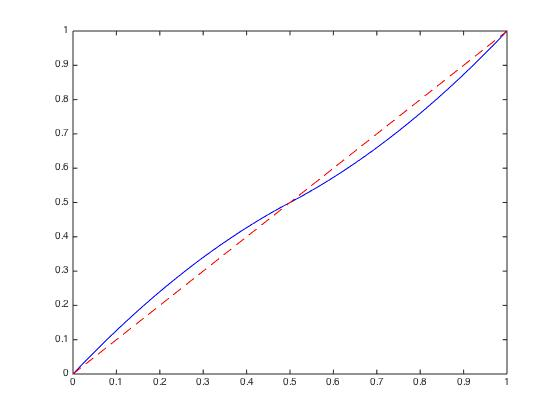
\includegraphics[width=8cm]{results/Probability_weighting_function.jpg}
%   \scalebox{1.0}{\begin{tikzpicture}
%   \begin{axis}[width=8cm,height=7.35cm,legend pos=south east,
%            grid = major,
%            grid style={dashed, gray!30},
%            xmin=0,     % start the diagram at this x-coordinate
%            xmax=1,    % end   the diagram at this x-coordinate
%            ymin=0,     % start the diagram at this y-coordinate
%            ymax=1,   % end   the diagram at this y-coordinate
%            axis background/.style={fill=white},
%            ylabel={\large Weight $w(p)$},
%            xlabel={\large Probability $p$}
%            ]
%           \addplot[domain=0:0.5, red, thick] 
%              {2/3*(2*x - x*x)}; 
%            \addplot[domain=0.5:1, red, thick, smooth]           {1/3 + 2/3 * x*x}; 
%            \addlegendentry{$w(p)$}
%                  \addplot[domain=0:1, blue, thick]           {x}; 
%   \end{axis}
%   \end{tikzpicture}}\\[1ex]
% }
% \caption{Weight function}
% \label{fig:w1}% \end{minipage}
% \end{figure}
% 
% 
% \paragraph{Background.}
% Let $X_1,\ldots, X_n$ be i.i.d. random variables with underlying distribution $U[0,5]$.  
% Then, the empirical distribution function is defined as
% \begin{align}
% {\hat F_n}(x)= \frac{1}{n} \sum_{i=1}^n 1_{(X_i \leq x)}.
% \label{eq:edf}
% \end{align}
% Thus,  $1-{\hat F_n}(x)$ is an unbiased estimator of $P(X>x)$. 
% From \eqref{eq:edf}, it is clear that ${\hat F_n}(x)$ generates a Lebesgue Stieljes measure which takes mass $\frac{1}{n}$ at each of the points $X_i, i=1,\ldots,n$. So does $w(1-{\hat F_n}(x))$. Based on this observation, one can see the weight function equivalently as follows:
% $$ w(1-{\hat F_n}(x)) =\int_x^{\infty} d w(1-{\hat F_n}(y))$$
% 
% % Observe also that the integral 
% % $$
% % \int_0^{+\infty} \wfn dx(\omega)
% % $$
% % always exists because $w^+$ is bounded and $\wfn$ takes values in a finite support.
% 
% Hence, the estimate $\widehat{V_n}(X)$ of $\C(X)$ is arrived at as follows:
% \begin{align}
% \widehat V_n(X)= \int_0^{\infty} w(1-{\hat F_n}(x)) dx=& - \intinfinity  \int_x^\infty d w(1-{\hat F_n}(y)) \\
% =& - \intinfinity  x d w(1-\hat{F_n}(x))\nonumber\\
% =&\sum_{i=1}^n X_{[i]} \left(w\left(\frac{i+1}{n}\right)- w\left(\frac{i}{n}\right)\right),\label{eq:c1}
% \end{align}
% where $X_{[i]}$ denotes the $i$th order statistic of the sample set $\{X_1,\ldots,X_n\}$. Note that, we let $w^+\left(\frac{n+1}{n}\right)=1$, $\forall n$.
% 
% We use \eqref{eq:c1} to estimate the CPT-value $\C(X)$. Analytically, $\C(X)=2.5$ for a $U[0,5]$ distributed random variable $X$.
% In the following, we report the accuracy of the estimator $\widehat{V}_n(X)$ using simulation experiments.
% 
%  \begin{figure}
%     \centering
% \tabl{c}{\scalebox{1.0}{\begin{tikzpicture}
% \begin{axis}[xlabel={number of samples $n$},ylabel={$\left| \overline \C_n - \C(X) \right|$}, width=8cm,height=7.35cm,ytick pos=left,xtick pos=left,grid,grid style={gray!30}]
% \addplot table[x index=0,y index=1,col sep=comma] {results/finaldata.txt};
% %\addlegendentry{$\l\theta_{k} - \hat\theta_T\r^2$}% y index+1 since humans count from 1
% \end{axis}
% \end{tikzpicture}}\\[1ex]}
% \caption{Weight function and estimation error for a $U[0,5]$ random variable.}
% \label{fig:perf}
% \end{figure}
% %In order to visualize the convergence rate of the empirical estimation scheme in \eqref{eq:cpt-est}, we set up $1000$ macro-simulations, with the number of samples used ranging from $100$ to $100,000$. 
% \paragraph{Results.} Fig. \ref{fig:perf} shows the estimation error obtained for a random variable $X$ with distribution $U[0.5]$. Here, the estimation error denotes the absolute difference between the estimated CPT-value \eqref{eq:c1} and true CPT-value, which is $2.5$. 
% From Fig. \ref{fig:perf}, it is evident that the CPT-value estimation scheme \eqref{eq:c1} converges rapidly to the true CPT-value.
% 
%%%%%%%%%%%%%%%%%%%%%%%%%%%%%%%%%%%%%%%%%%%%%%%%%%%%%%%%%%%%%%
%%%%%%%%%%%%%%%%%%%%%%%%%%%%%%%%%%%%%%%%%%%%%%%%%%%%%%%%%%%%%%
%%%%%%%%%%%%%%%%%%%%%%%%%%%%%%%%%%%%%%%%%%%%%%%%%%%%%%%%%%%%%%
%%%%%%%%%%%%%%%%%%%%%%%%%%%%%%%%%%%%%%%%%%%%%%%%%%%%%%%%%%%%%%
%%%%%%%%%%%%%%%%%%%%%%%%%%%%%%%%%%%%%%%%%%%%%%%%%%%%%%%%%%%%%%

\section{Conclusions and Future Work}
\label{sec:conclusions}
CPT has been a very popular paradigm for modeling human decisions among psychologists/economists, but has escaped the radar of the AI community. This work is the first step in incorporating CPT-based criteria into an RL framework. However, both estimation and control of CPT-based value is challenging. Using temporal-difference learning type algorithms for estimation was ruled out for CPT-value since the underlying probabilities get (non-linearly) distorted by a weight function. Using empirical distributions, we proposed an estimation scheme that converges at the optimal rate. Next, for the problem of control, since CPT-value does not conform to any Bellman equation, we employed SPSA - a popular simulation optimization scheme and designed both first and second-order algorithms for optimizing the CPT-value function. 
We provided theoretical convergence guarantees for all the proposed algorithms. We illustrated the usefulness of CPT-based criteria in a numerical example.

%%%%%%%%%%%%%%%%%%%%%%%%%%%%%%%%%%%%%%%%%%%%%%%%%%%%%%%%%%%%

\bibliographystyle{plainnat}

% \bibliographystyle{jsr}
\bibliography{cpt-refs}

\end{document}


